\chapter{Evaluation}
\label{sec.Evaluation}
Dieses Kapitel behandelt die Evaluation der nach den in Kapitel \ref{sec.Methodik} beschriebenen Schritten erstellten binären und quantitativen Modellen. In einem ersten Schritt werden die zur Modellerstellung benutzten Datensätze vorgestellt (Abschnitt \ref{sec.Datensätze}). Darauf aufbauend erfolgt eine Einführung der Fehlermaße (Abschnitt \ref{sec.Beschreibung der Fehlermaße}) für das binäre sowie das quantitative Modell, mit denen die Prädiktionsgenauigkeiten beider Modelle bewertet werden können. Die Bewertung der Modelle erfolgt separat für den binären Fall (Abschnitt \ref{sec.Binäres Modell}) und den quantitativen Fall (Abschnitt \ref{sec.Quantitatives Modell}). Es werden Vergleiche der Modelle gegenüber statischen Repräsentationen von Personen-Auftrittswahrscheinlichkeiten (binäres Modell) sowie Personenraten (quantitatives Modell) gezogen. Im Rahmen dieser Vergleiche werden außerdem limitierende Modellfaktoren erörtert. \\
\section{Datensätze}
\label{sec.Datensätze}
Zur Evaluation der in dieser Arbeit präsentierten Methoden dienen zwei separate Datensätze. Für den im Folgenden als  \glqq Aruba-Datensatz\grqq{} bezeichneten Datensatz wurde über einen Zeitraum von 16 Wochen das Personenaufkommen innerhalb einer Wohnung aufgezeichnet \cite{aruba}. Hierbei wurde die Wohnung in insgesamt zehn verschiedene Räume aufgeteilt und minütlich der Aufenthaltsort einer Person dokumentiert. Als Beschränkung gilt, dass sich zu jedem Zeitpunkt nur maximal eine Person in der Wohnung befinden konnte. Befand sich die Person außerhalb der Wohnung, so ist dies im Datensatz als Raum \glqq Outside\grqq{} dokumentiert.
Die in den folgenden Abschnitten durchgeführten Untersuchungen beruhen stets auf einem Modell, welches mittels der Daten der ersten zwölf der insgesamt 16 Wochen nach den Gleichungen \ref{eq:Inkrementelle Fouriertransformation} trainiert wurde. Jeder der zehn Räume ist dabei durch eine einzelne Zelle repräsentiert. Zur Evaluation des Modells wird der Prädiktionsfehler $\epsilon_\ind{p}$ für die letzten vier Wochen des Datensatzes berechnet. Als Modellordnung $l_\ind{opt}$ wird, wie schon in Abschnitt \ref{sec.Verarbeitung server binär} beschrieben, die Ordnung mit dem geringsten Prädiktionsfehler $\epsilon_\ind{p,opt}$ gewählt.  \\
% Hier die Quelle von dem Datensatz einfügen?
Der zweite Datensatz, im Folgenden als \glqq {UOL-Datensatz}\grqq{} bezeichnet, wurde durch einen, an einer statischen Position befindlichen, 3D-Laserscanner innerhalb eines Bürokomplexes des Isaac Newton Building der University of Lincoln (UOL) aufgenommen \cite{uol}. Über einen Zeitraum von 22 aufeinanderfolgenden Tagen, beginnend mit dem 23. November 2018, wurden mit einer Frequenz von $\SI{0.5}{\hertz}$ Personendetektionen mit den zugehörigen Zeitstempeln und Positionsdaten innerhalb einer Umgebung mit einer Gesamtfläche von ca. \SI{85}{\metre\squared} aufgezeichnet \cite{uol}. Zur Modellberechnung in den folgenden Abschnitten wird über das Bürogebäude ein Gitter mit den Maßen $\SI{30}{\metre} \, \mathrm{x} \, \SI{25.5}{\metre}$ gelegt. Jede Zelle innerhalb des Gitters hat die Maße $\SI{0.5}{\metre} \, \mathrm{x} \, \SI{0.5}{\metre}$, sodass man insgesamt 3060 verschiedene Zellen erhält. Die ersten zwei Wochen des Datensatzes werden für die Erstellung des Modells verwendet. Zur Evaluierung wird $\epsilon_\ind{p}$ mittels der Daten der dritten Woche berechnet. Als Modellordnung wird auch hier die Ordnung $l_\ind{opt}$ mit dem geringsten Prädiktionsfehler $\epsilon_\ind{p,opt}$ gewählt. 

\section{Beschreibung der Fehlermaße}
\label{sec.Beschreibung der Fehlermaße}
Um die Prädiktionsgenauigkeit der Modelle bewerten zu können, ist ein einheitliches Fehlermaß notwendig. Im Folgenden werden daher sowohl für das binäre wie auch für das quantitative Modell Fehlermaße eingeführt, welche in einem späteren Abschnitt dieses Kapitels für Vergleiche mit statischen Modellen herangezogen werden.
\subsection{Fehlermaße des binären Modells}
\label{sec.Fehlermaße binäres Modell}
Für die Bewertung der Modelle wird ein einheitliches Fehlermaß benutzt. Wie schon in Abschnitt \ref{sec.Beschreibung binärer Zustandsmodelle} beschrieben und auch in \cite{Krajnik.2014} erwähnt, führt eine Erhöhung der Modellordnung dazu, dass die zur Erstellung des Modells verwendeten Daten besser abgebildet werden können. Der Rekonstruktionsfehler $\epsilon_\ind{r}$ sinkt. Der Einfluss auf den Prädiktionsfehler $\epsilon_\ind{p}$, also die Genauigkeit, mit der zukünftige Zellzustände modelliert werden können, ist jedoch komplexer.
Grafisch dargestellt ist dies in \bild{prediction_vs_estimation_error}.
% Achsbeschriftungen in Prozent umschreiben
\begin{figure}[!h]
	\centering
	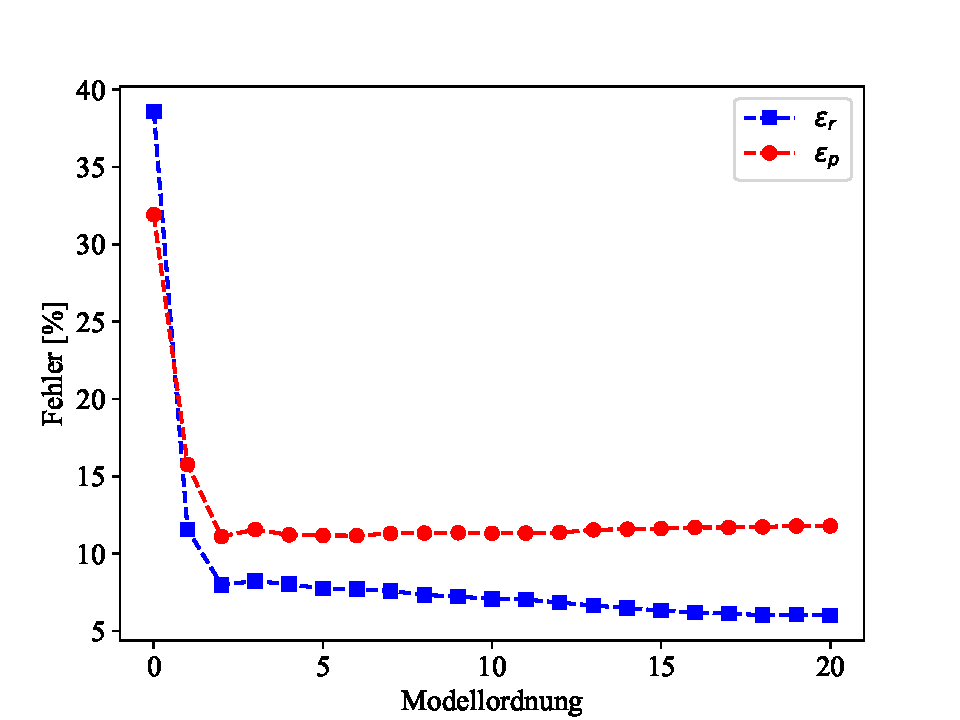
\includegraphics[width=0.7\linewidth]{Abbildungen/evaluation/prediction_vs_estimation_error}
	\caption{Rekonstruktionsfehler $\epsilon_\ind{r}$ und Prädiktionsfehler $\epsilon_\ind{p}$ mit steigender Modellordnung}
	\label{fig.prediction_vs_estimation_error}
\end{figure}

Zur Bewertung der Modellgenauigkeiten wird in den folgenden Abschnitten stets die Modellordnung $l_\ind{opt}$ mit dem geringsten Prädiktionsfehler $\epsilon_\ind{p,opt}$ gewählt. Der Fehler berechnet sich dabei nach Gleichung \ref{eq:Prädiktionsfehler}. Die maximale Modellordnung wird zu $l_\ind{max} = 20$ gesetzt. Der Schwellwert zur Ermittlung des prognostizierten Zellzustandes $s'(t)$ mittels der Zellwahrscheinlichkeitsfunktion $p(t)$ beträgt $c = 0.5$ (siehe Gleichung \ref{eq:Schwellwert-Verfahren}).

\subsection{Fehlermaße quantitatives Modell}
\label{sec.Fehlermaße quantitatives Modell}
Die optimale Modellordnung $l_\ind{opt}$ des quantitativen Modells berechnet sich ebenfalls durch die Minimierung des Prädiktionsfehlers $\epsilon_\ind{p}$. Da für den quantitativen Fall jedoch die Personenraten $\lambda' (t)$ für die einzelnen Intervalle $\Delta t_i$ berechnet werden, erfolgt die Ermittlung des Prädiktionsfehlers nach Gleichung \ref{eq:Prädiktionsfehler quantitativ}.
% In Kapitel Methodik noch die Berechnung vom Prädiktionsfehler nach lsme-Methode reinschreiben.
Die Rate $\lambda ' (t)$ wird auf die nächste natürliche Zahl gerundet, damit sichergestellt ist, dass $\lambda ' (t) \in \mathbb{N}$ gilt. Die maximale Modellordnung wird zu $l_\ind{max} = 20$ gesetzt.
\section{Binäres Modell}
\label{sec.Binäres Modell}
In diesem Abschnitt erfolgt eine Evaluation des binären Modells. Untersucht wird das Modell bei unterschiedlichen Intervalldauern $\Delta t$. Für den binären Fall berechnen sich die Personendetektionen im $n$-ten Zeitintervall (siehe Gleichung \ref{eq:Detektionen pro Intervall}) zu

\begin{equation}\label{eq:Fallunterscheidung a_n}
	a_n = \begin{cases}
		1 & , \qquad a_n \geq 1 \\
		0 & , \qquad a_n < 1 \, 
	\end{cases} .
\end{equation}

Die Einteilung der gesamten Periodendauer, wie beispielsweise einer Woche, in unterschiedlich lange Intervalldauern, resultiert aus der Tatsache, dass ein mobiler Roboter im Normalfall keine komplette Übersicht über die zu modellierende Umgebung $\mathcal{U}$ besitzt. Mit einer Vergrößerung der Intervalldauer soll sichergestellt werden, dass der Roboter innerhalb dieser Dauer die Umgebung $\mathcal{U}$ mindestens einmal komplett abfahren kann. Begründet werden kann dies damit, dass im vorliegenden Modell das Nicht-Beobachten einer Zelle einer Nicht-Detektion von Personen entspricht. Wird während eines Intervalls mindestens eine Person detektiert, so wird der Zellenstatus im entsprechenden Intervall auf $s(t) = 1$ gesetzt. Die Dauer des Aufenthaltes des Roboters in einer Zelle innerhalb eines Intervalls kann nicht berücksichtigt werden. Je nach Umgebungsgröße und Detektionsbereich des mobilen Roboters sollte die Intervalldauer angepasst werden. Die Summe an Zeitstempeln innerhalb der Periodendauer reduziert sich mit steigender Intervalldauer $\Delta t$ und geht somit mit einem Informationsverlust einher. Der Zellzustand $s(t)$ bei unterschiedlichen Intervalldauern $\Delta t$ ist in \bild{bin_size_influence_master_bedroom_binary} dargestellt. 


\begin{figure}[!h]
		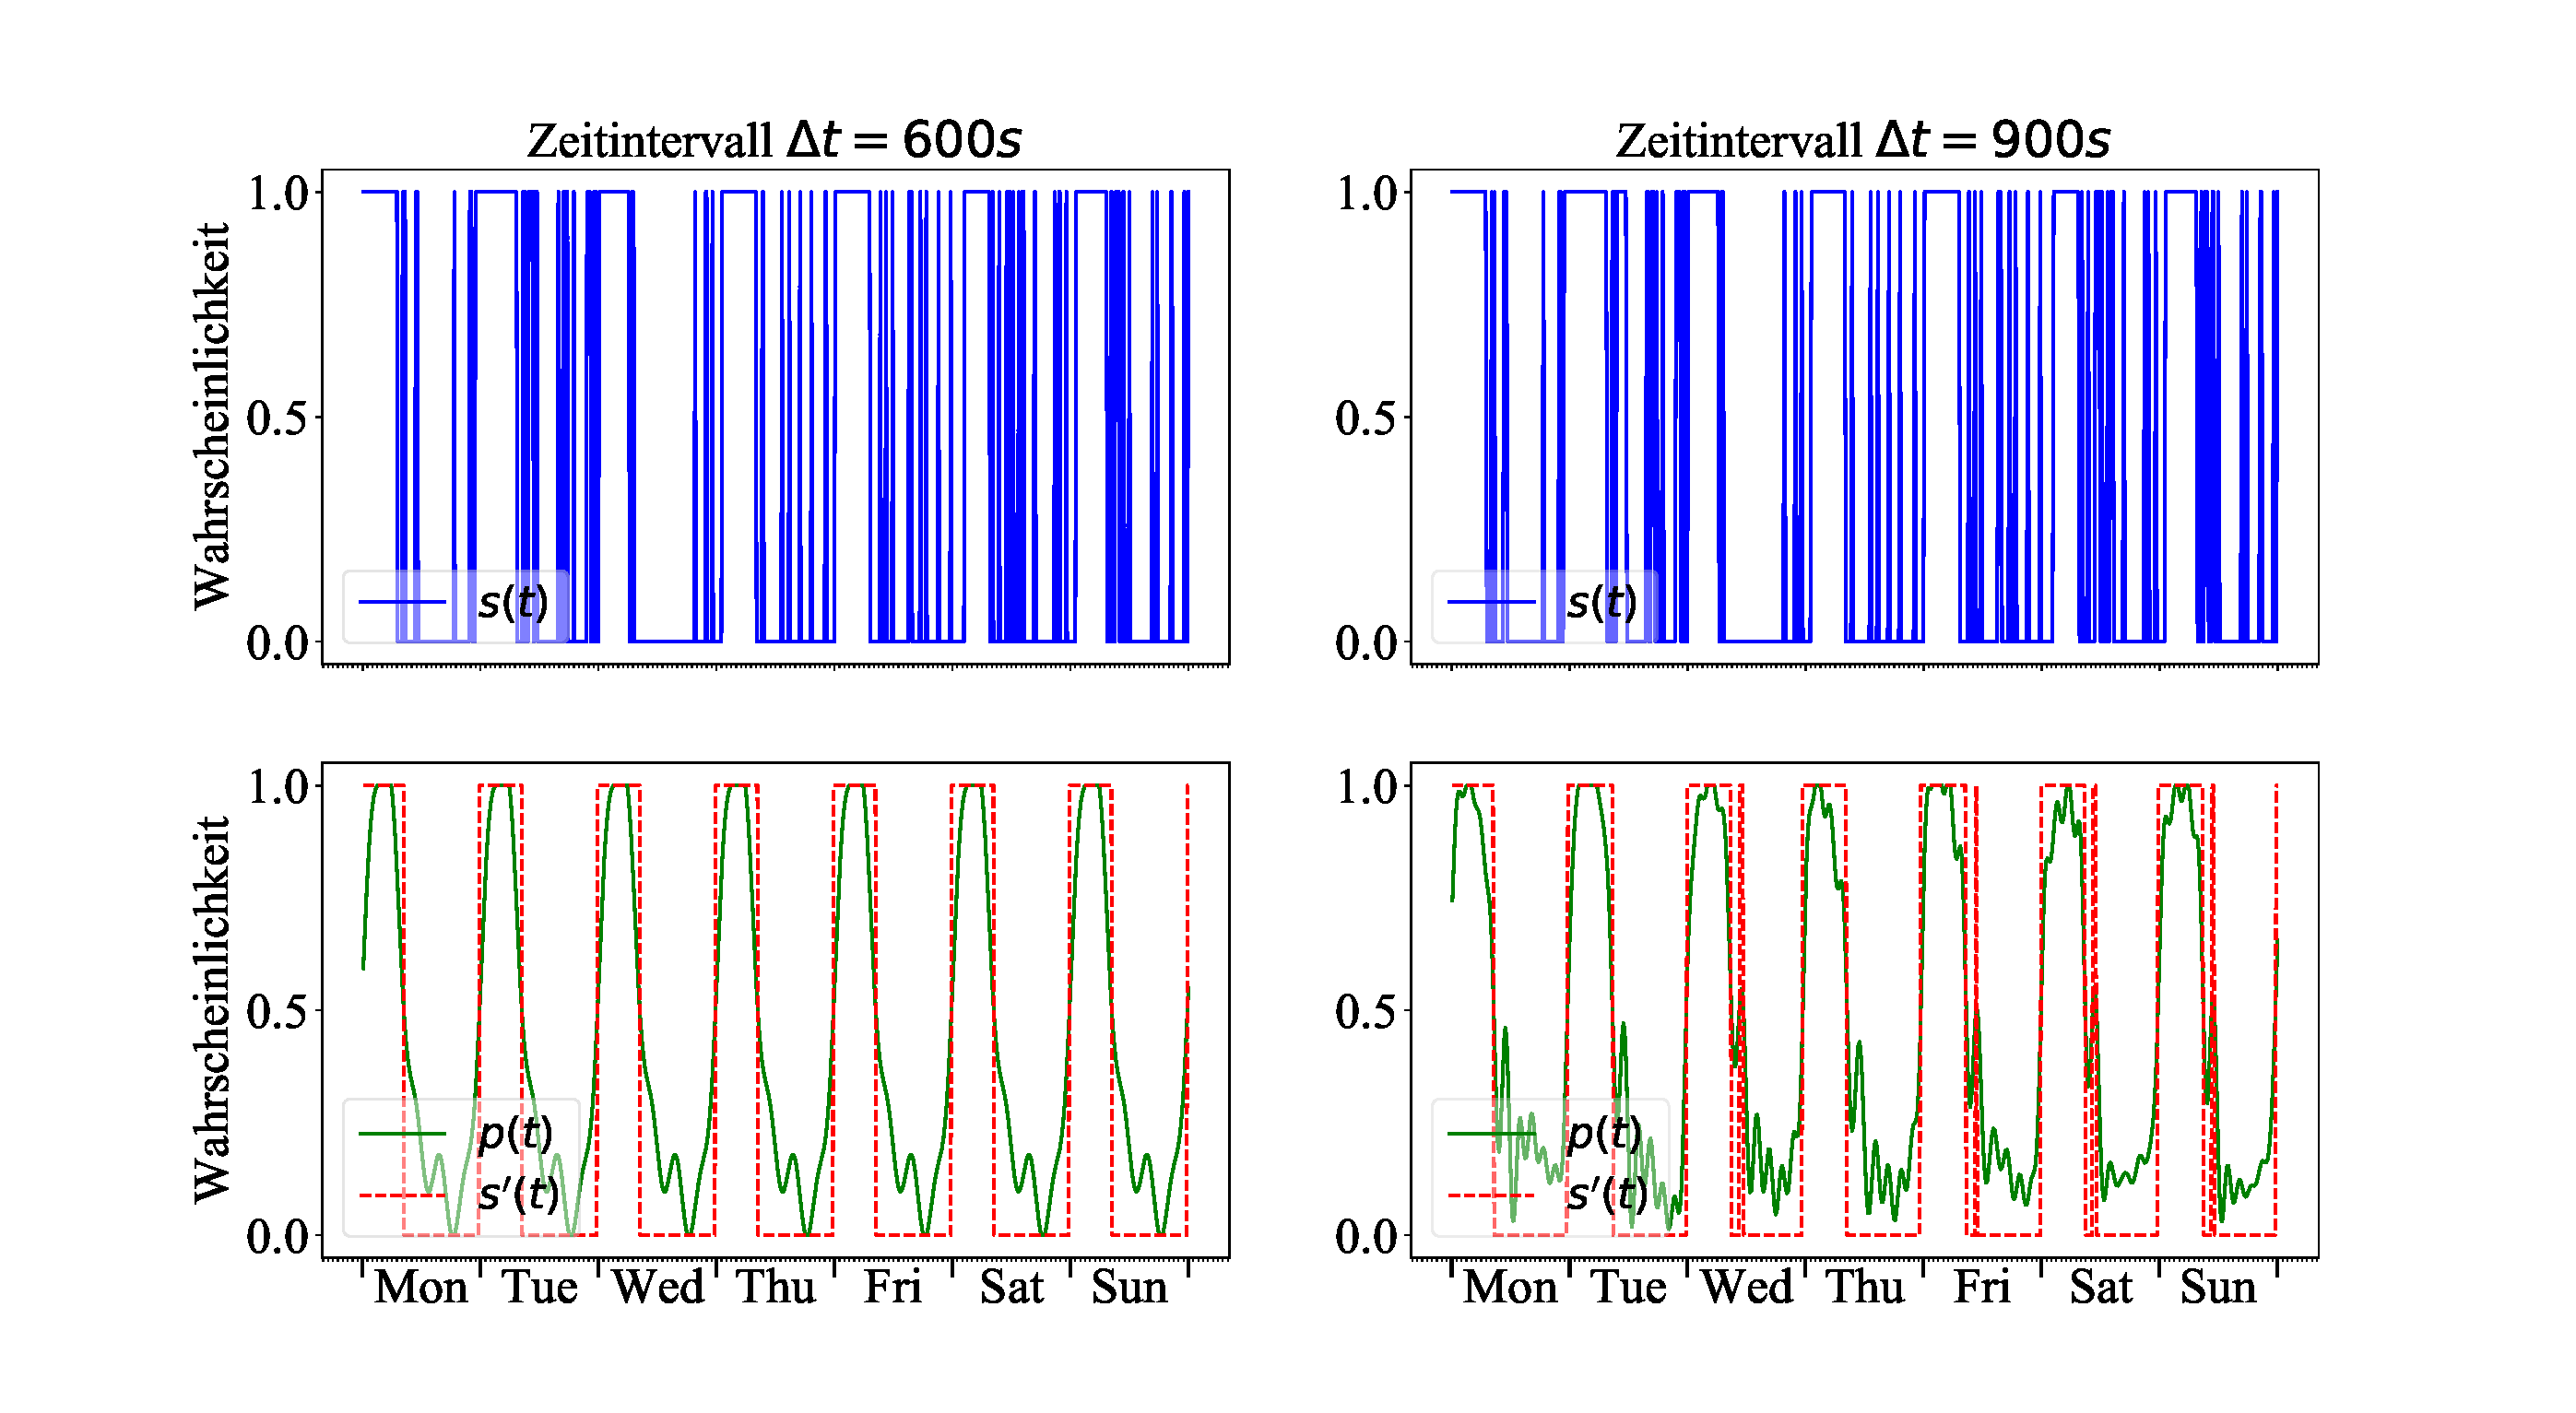
\includegraphics[width=\linewidth]{Abbildungen/evaluation/bin_size_influence_master_bedroom_binary.pdf}
		\caption[Zellzustand $s(t)$ sowie Wahrscheinlichkeitsfunktion $p(t)$ und prognostizierter Zellzustand $s'(t)$ des Schlafzimmers des Apartments mit einer Intervalldauer von $\Delta t = \SI{600}{\second}$ und $\Delta t = \SI{900}{\second}$]{Zellzustand $s(t)$ sowie Wahrscheinlichkeitsfunktion $p(t)$ und prognostizierter Zellzustand $s'(t)$ des Schlafzimmers des Apartments (Aruba-Datensatz) mit einer Intervalldauer von $\Delta t = \SI{600}{\second}$ (links) und $\Delta t = \SI{900}{\second}$ (rechts)}
		\label{fig.bin_size_influence_master_bedroom_binary}
\end{figure}

% Hier Abbildung einfügen von Master-Bedroom
Betrachtet wird hier das Schlafzimmer des Apartments des Aruba-Datensatzes. 
Die beiden Grafiken auf der linken Seite zeigen den Zellzustand $s(t)$ (oben) über einen Gesamtzeitraum von einer Woche für eine Intervalldauer von $\Delta t = \SI{600}{\second} $, die Wahrscheinlichkeitsfunktion $p(t)$ der Zelle sowie der anhand des Schwellwertes $c = 0.5$  prognostizierte Zellzustand $s'(t)$. Auf der rechten Seite von \bild{bin_size_influence_master_bedroom_binary} ist der Zellzustand $s(t)$ für eine Intervalldauer von $\Delta t = \SI{900}{\second}$ sowie die Wahrscheinlichkeitsfunktion der Zelle und der prognostizierte Zellzustand $s'(t)$ aufgetragen. Während zur Bestimmung von $p(t)$ im Falle von $\Delta t = \SI{600}{\second} $ eine Modellordnung von $l_\ind{opt} =2$ einen Prädiktionsfehler von $\epsilon_\ind{p,opt} = 17.8 \% $ erreicht,
beträgt die optimale Modellordnung $l_\ind{opt} =3$ bei einer Intervalldauer von $\Delta t = \SI{900}{\second}$  mit einem Prädiktionsfehler  von $\epsilon_\ind{p,opt} = 7.4 \% $. Hierbei ist anzumerken, dass aus den obigen Ergebnissen nicht geschlossen werden kann, dass eine Intervalldauer von $\Delta t = \SI{900}{\second}$ ein genaueres Modell erzeugt als eine Intervalldauer von $\Delta t = \SI{600}{\second}$. Die Ergebnisse der unterschiedlichen Intervalle sind nicht miteinander vergleichbar. Eine höhere Intervalldauer geht mit einer größeren Wahrscheinlichkeit mindestens einer Personendetektion einher. Somit steigt der Anteil an Intervallen, in denen Personendetektionen vorliegen, gegenüber der Gesamtanzahl an Zeitintervallen. Wie bereits am Anfang dieses Abschnittes erwähnt, geht eine Vergrößerung der Intervalldauer $\Delta t$ immer auch mit einem Informationsverlust einher. Eine Bewertung der Modelle kann jedoch durch den Vergleich mit den zugehörigen statischen Modellen gezogen werden.  Für den statischen Fall, also die Annahme einer konstanten Wahrscheinlichkeit $p_\ind{stat}(t) = \mathrm{const}.\, $, ergibt sich $\epsilon_\ind{p,stat} = 40.5 \%$ für eine Intervalldauer von $\Delta t = \SI{600}{\second}$, der statische Prädiktionsfehler bei einer Intervalldauer von $\Delta t = \SI{900}{\second}$ berechnet sich zu $\epsilon_\ind{p,stat} = 44.3 \%$. Die größere Intervalldauer spiegelt sich in dem Modell derart wider, dass die Anzahl der Personendetektionen im Verhältnis zu der Anzahl $n$ der Zeitstempel zunimmt, und die Breite der rot gestrichelten Balken, welche Phasen einer durchgängigen Zellbelegtheit signalisieren, in \bild{bin_size_influence_master_bedroom_binary} zunimmt.\\
Eine Limitation der Methode ist jedoch in \bild{bin_size_influence_second_bedroom_binary} zu sehen. Betrachtet wird der Zellzustand $s(t)$ des Gästeschlafzimmers innerhalb des Apartments.

\begin{figure}[!h]
	\begin{center}
		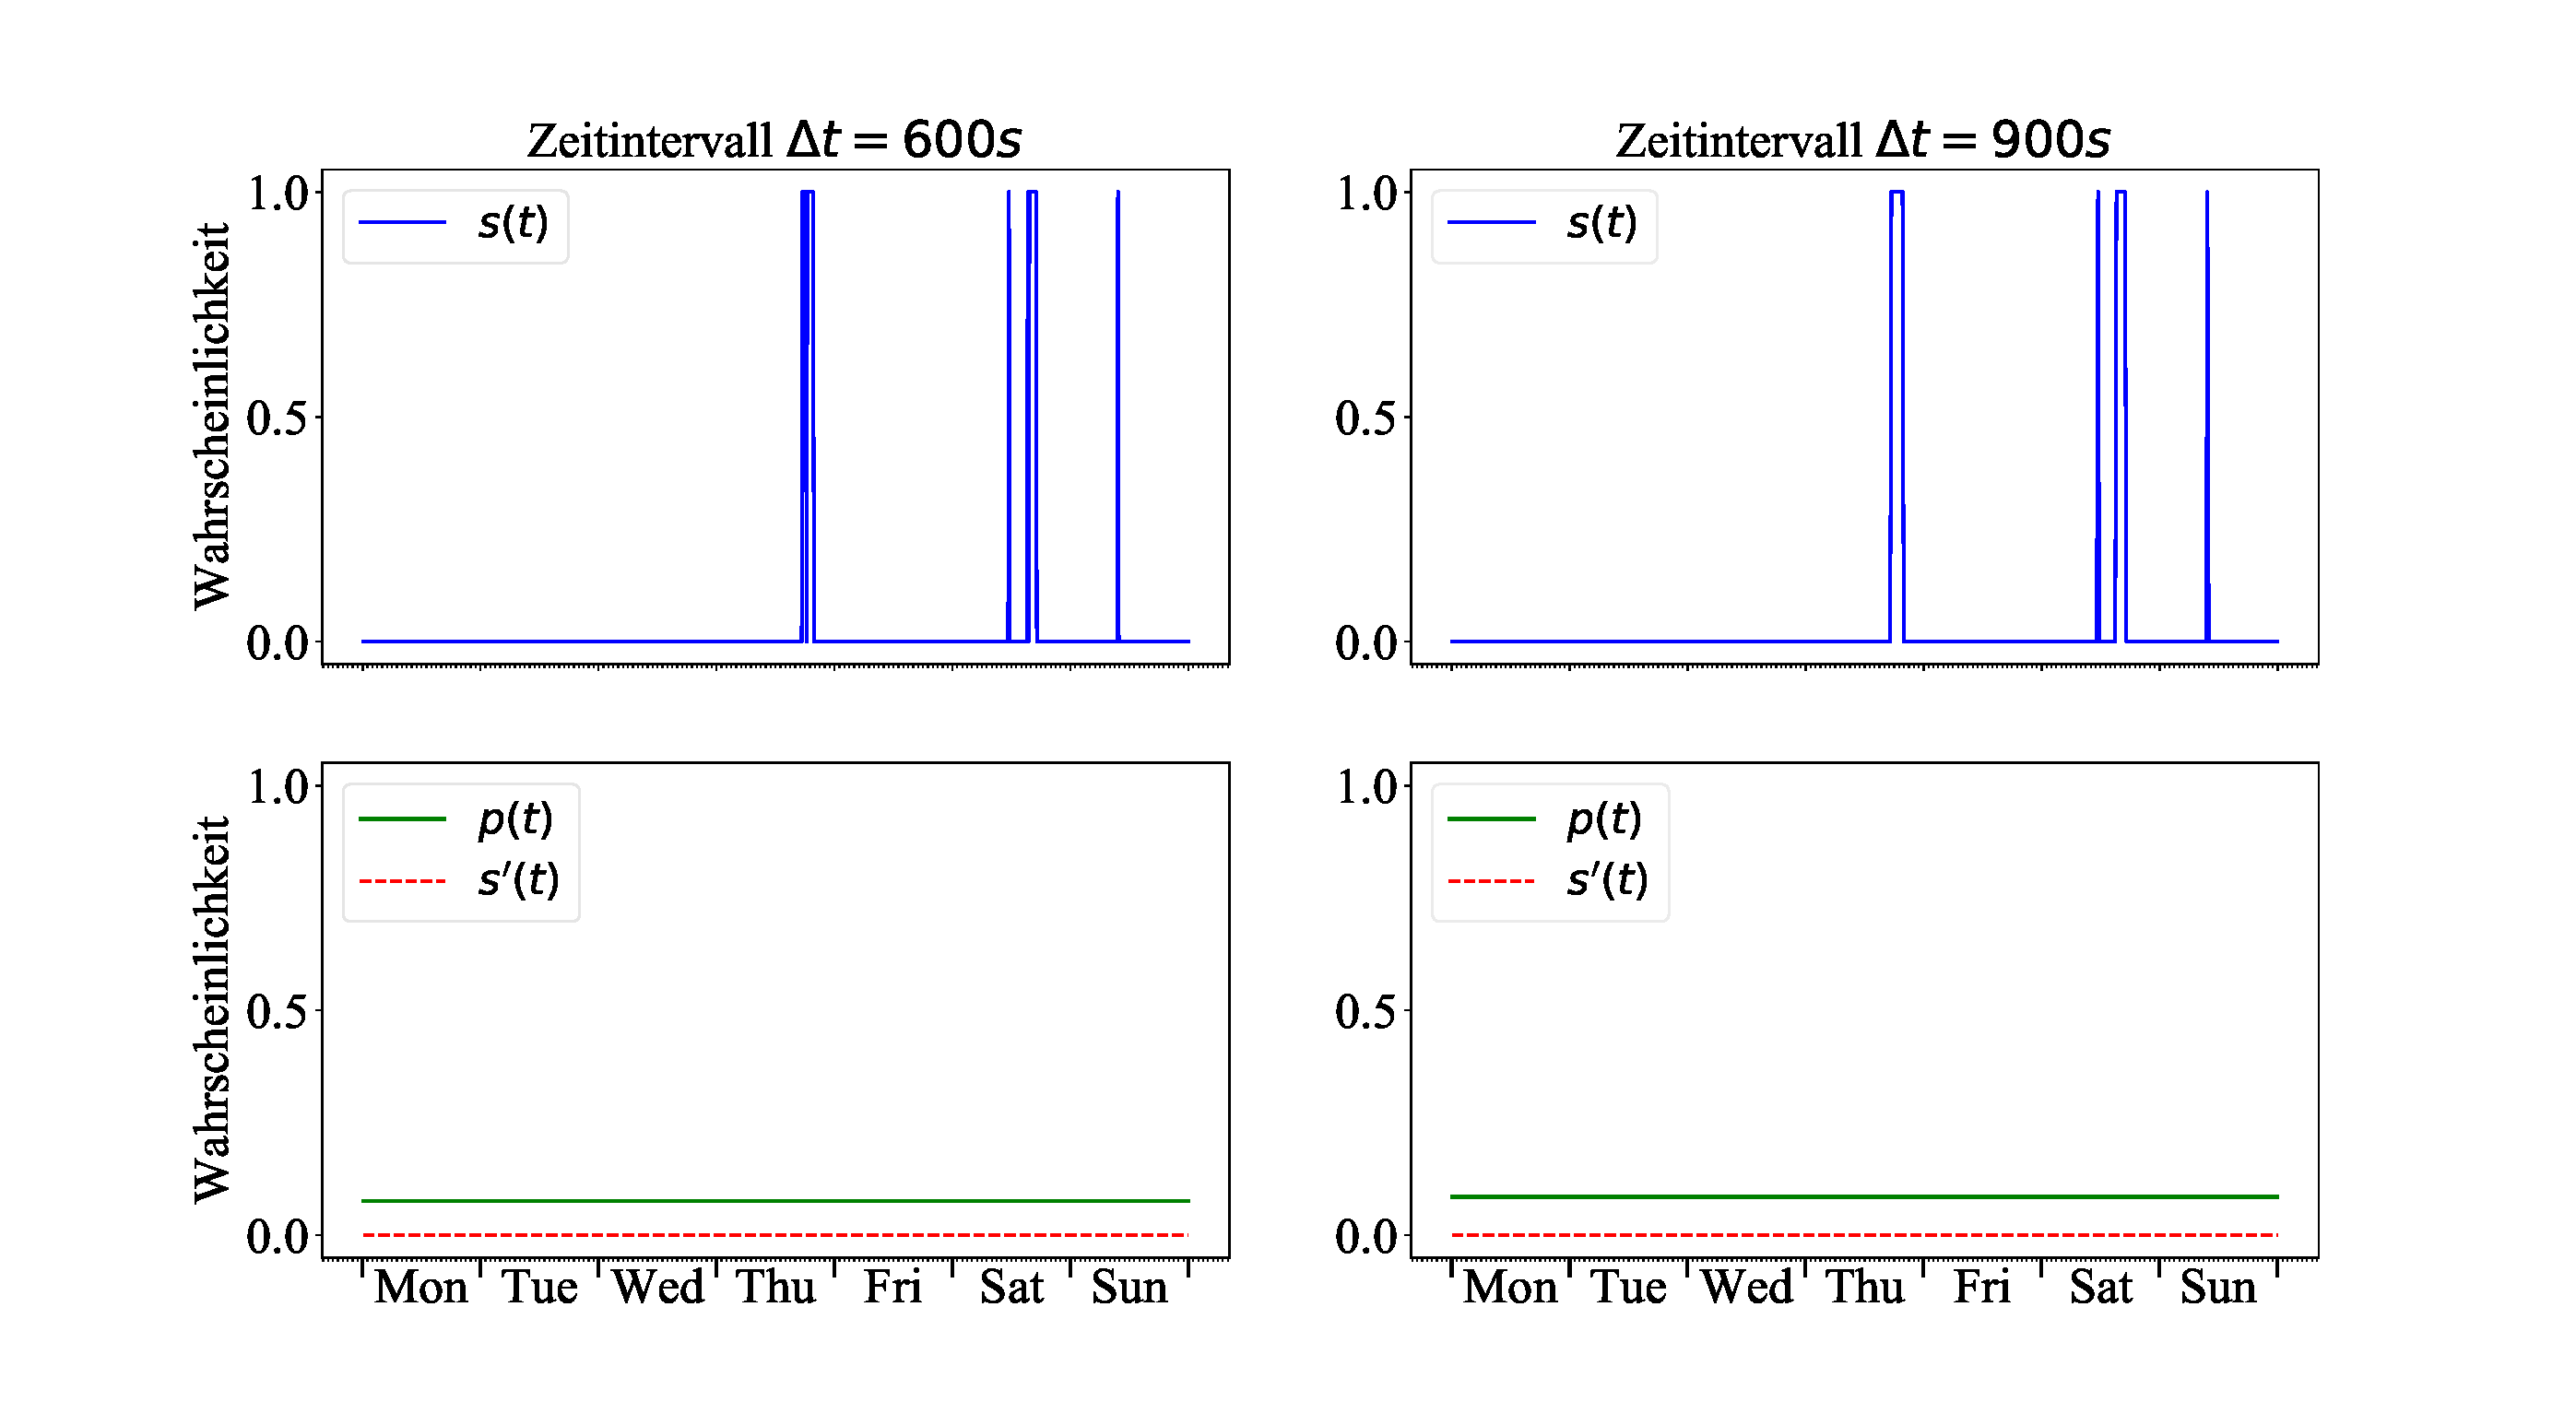
\includegraphics[width=\linewidth]{Abbildungen/evaluation/bin_size_influence_second_bedroom_binary.pdf}
		\caption[Zellzustand $s(t)$ sowie Wahrscheinlichkeitsfunktion $p(t)$ und prognostizierter Zellzustand $s'(t)$ des Gästeschlafzimmers des Apartments mit einer Intervalldauer von $\Delta t = \SI{600}{\second}$ und $\Delta t = \SI{900}{\second}$]{Zellzustand $s(t)$ sowie Wahrscheinlichkeitsfunktion $p(t)$ und prognostizierter Zellzustand $s'(t)$ des Gästeschlafzimmers des Apartments (Aruba-Datensatz) mit einer Intervalldauer von $\Delta t = \SI{600}{\second}$ (links) und $\Delta t = \SI{900}{\second}$ (rechts)}
		\label{fig.bin_size_influence_second_bedroom_binary}
	\end{center}
\end{figure}

Bei einer Intervalldauer von $\Delta t = \SI{600}{\second}$ ergibt sich die, nach Gleichung \ref{eq:Prädiktionsfehler}, optimale Modellordnung zu $l_\ind{opt}=0$, dargestellt durch die konstante, statische Wahrscheinlichkeitsfunktion $p_\ind{stat}(t)$. Zu dem selben Ergebnis kommt man bei einer Intervalldauer von $\Delta t = \SI{900}{\second}$. Auch hier beträgt die optimale Modellordnung $l_\ind{opt}=0$. Durch die Erhöhung der Personendetektionen im Vergleich zur Anzahl der Zeitstempel liegt die statische Wahrscheinlichkeit einer Personendetektion in der rechten, unteren Grafik von \bild{bin_size_influence_second_bedroom_binary} bei $p_\ind{stat}(t) = 7.9 \%$, während in der unteren linken Grafik $p_\ind{stat}(t) = 7.5 \%$ gilt. Die Personendetektionen beschränken sich auf seltene, kurzperiodige Bereiche, welche nicht durch die maximale Modellordnung von $l_\ind{max} = 20$ modelliert werden können. Eine weitere Erhöhung der Modellordnung würde dazu führen, dass der Rekonstruktionsfehler $\epsilon_\ind{r}$ zwar sinken würde, die Generalisierungsfähigkeit des Modells jedoch verloren geht und es in der Folge zu einem Anstieg des Prädiktionsfehlers $\epsilon_\ind{p}$ kommt. Der Prädiktionsfehler des statischen Modells bei einer Intervalldauer von $\Delta t = \SI{600}{\second}$ ergibt sich zu $\epsilon_\ind{p,stat} = 6.5 \%$, im Falle von $\Delta t = \SI{900}{\second}$ zu $\epsilon_\ind{p,stat} = 7.4 \% $. Erneut sei darauf hingewiesen, dass die Modelle mit den unterschiedlichen Intervalldauern nicht miteinander vergleichbar sind. Ein Vergleich kann lediglich gegenüber den zugehörigen, statischen Modellen, gezogen werden.\\
% Erklären: Warum ist das so? Grundbelegtheit nimmt durch Vergrößerung der Intervalle zu. Modell prognostiziert aber immer 0, sodass der Prädiktionsfehler steigt
Einen zusammenfassenden Überblick der Modellfehler gibt Tabelle \ref{tab.Prädiktionsfehler aruba_binary}.

\begin{table}[!h]
	\centering
	\caption{Prädiktionsfehler $\epsilon_\ind{p}$ bei unterschiedlichen Intervalldauern $\Delta t$ (Aruba)}\label{tab.Prädiktionsfehler aruba_binary}
	\vspace*{-3mm}
	\begin{tabular}{lcr}
		\toprule
		Intervalldauer $\Delta t$		& $\epsilon_\ind{p,opt}$ & $\epsilon_\ind{p,stat}$              \\
		\midrule
		\SI{300}{\second}	& 12.7 \%         & 20.4 \%  \\
		\rowcolor{Snow2}
		\SI{600}{\second} 	& 14.4 \%        & 23.42 \% \\
		\SI{900}{\second}   & 14.31 \%  & 22.99 \%	\\
		\bottomrule
	\end{tabular} 
\end{table}

Aufgeteilt nach unterschiedlichen Intervalldauern sind die Prädiktionsfehler $\epsilon_\ind{p}$ aller Zellen für die optimale Modellordnung $l_\ind{opt}$ sowie für den statischen Fall aufgeführt.
% Hier die Tabelle einfügen und noch ein paar Erläuterungen dazu äußern
Betrachtet werden jedoch nur Zellen bzw. Räume, welche während mindestens 5 \% der betrachteten Zeitintervalle $\Delta t_i$ belegt waren. Innerhalb des Aruba-Datensatzes erfüllen sieben der insgesamt zehn Zellen diese Anforderung. Die Begründung dieser Anforderung geht aus \bild{bin_size_influence_second_bedroom_binary} hervor. Die Modellierbarkeit kurzfristiger Zellenbelegtheiten ist limitiert. In diesen Fällen liegt das statische Modell mit einer prognostizierten, konstanten Zellenbelegtheit von $p(t) = \mathrm{const}. = 0$ bereits zu mindestens 95 \% richtig und würde so die Evaluierung der Methode verfälschen. Eine allgemeine Aussage über die optimale Modellordnung $l_\ind{opt}$ kann nicht getroffen werden. Wie in Abschnitt \ref{sec.Verarbeitung server binär} beschrieben wird, erstellt der Server für jede Zelle des Gitters ein separates Modell. Somit variiert auch die optimale Modellordnung je nach betrachteter Zelle. \\
% Anmerkung: ein sinnvoller Minimalwert kann glaube ich nicht angegeben werden, variiert ja von Modell zu Modell sehr stark
Eine weitere Evaluation erfolgt anhand des UOL-Datensatzes. Erneut werden die Modelle der insgesamt 3060 Zellen bei verschiedenen Intervalldauern $\Delta t$, in welche die Periodendauer $T$ eingeteilt wird, betrachtet. Wie in Abschnitt \ref{sec.Datensätze} erwähnt, werden zur Ermittlung der Modellparameter die Daten von zwei aufeinander folgenden Wochen benutzt. Die Ermittlung der optimalen Modellordnung $l_\ind{opt}$ mittels eines minimalen Prädiktionsfehlers $\epsilon_\ind{p,opt}$ erfolgt mit Daten einer weiteren, dritten Woche. \bild{bin_size_influence_cell_row_23_col_25_binary} zeigt die binären Modelle bei einer Intervalldauer von $\Delta t = \SI{600}{\second} $ (links) sowie für $\Delta t = \SI{900}{\second} $ (rechts). 
% Hier Abbildung bin_size_influence_cell_row_23_col_25_binary.pdf einfügen
\begin{figure}[!h]
	\centering
	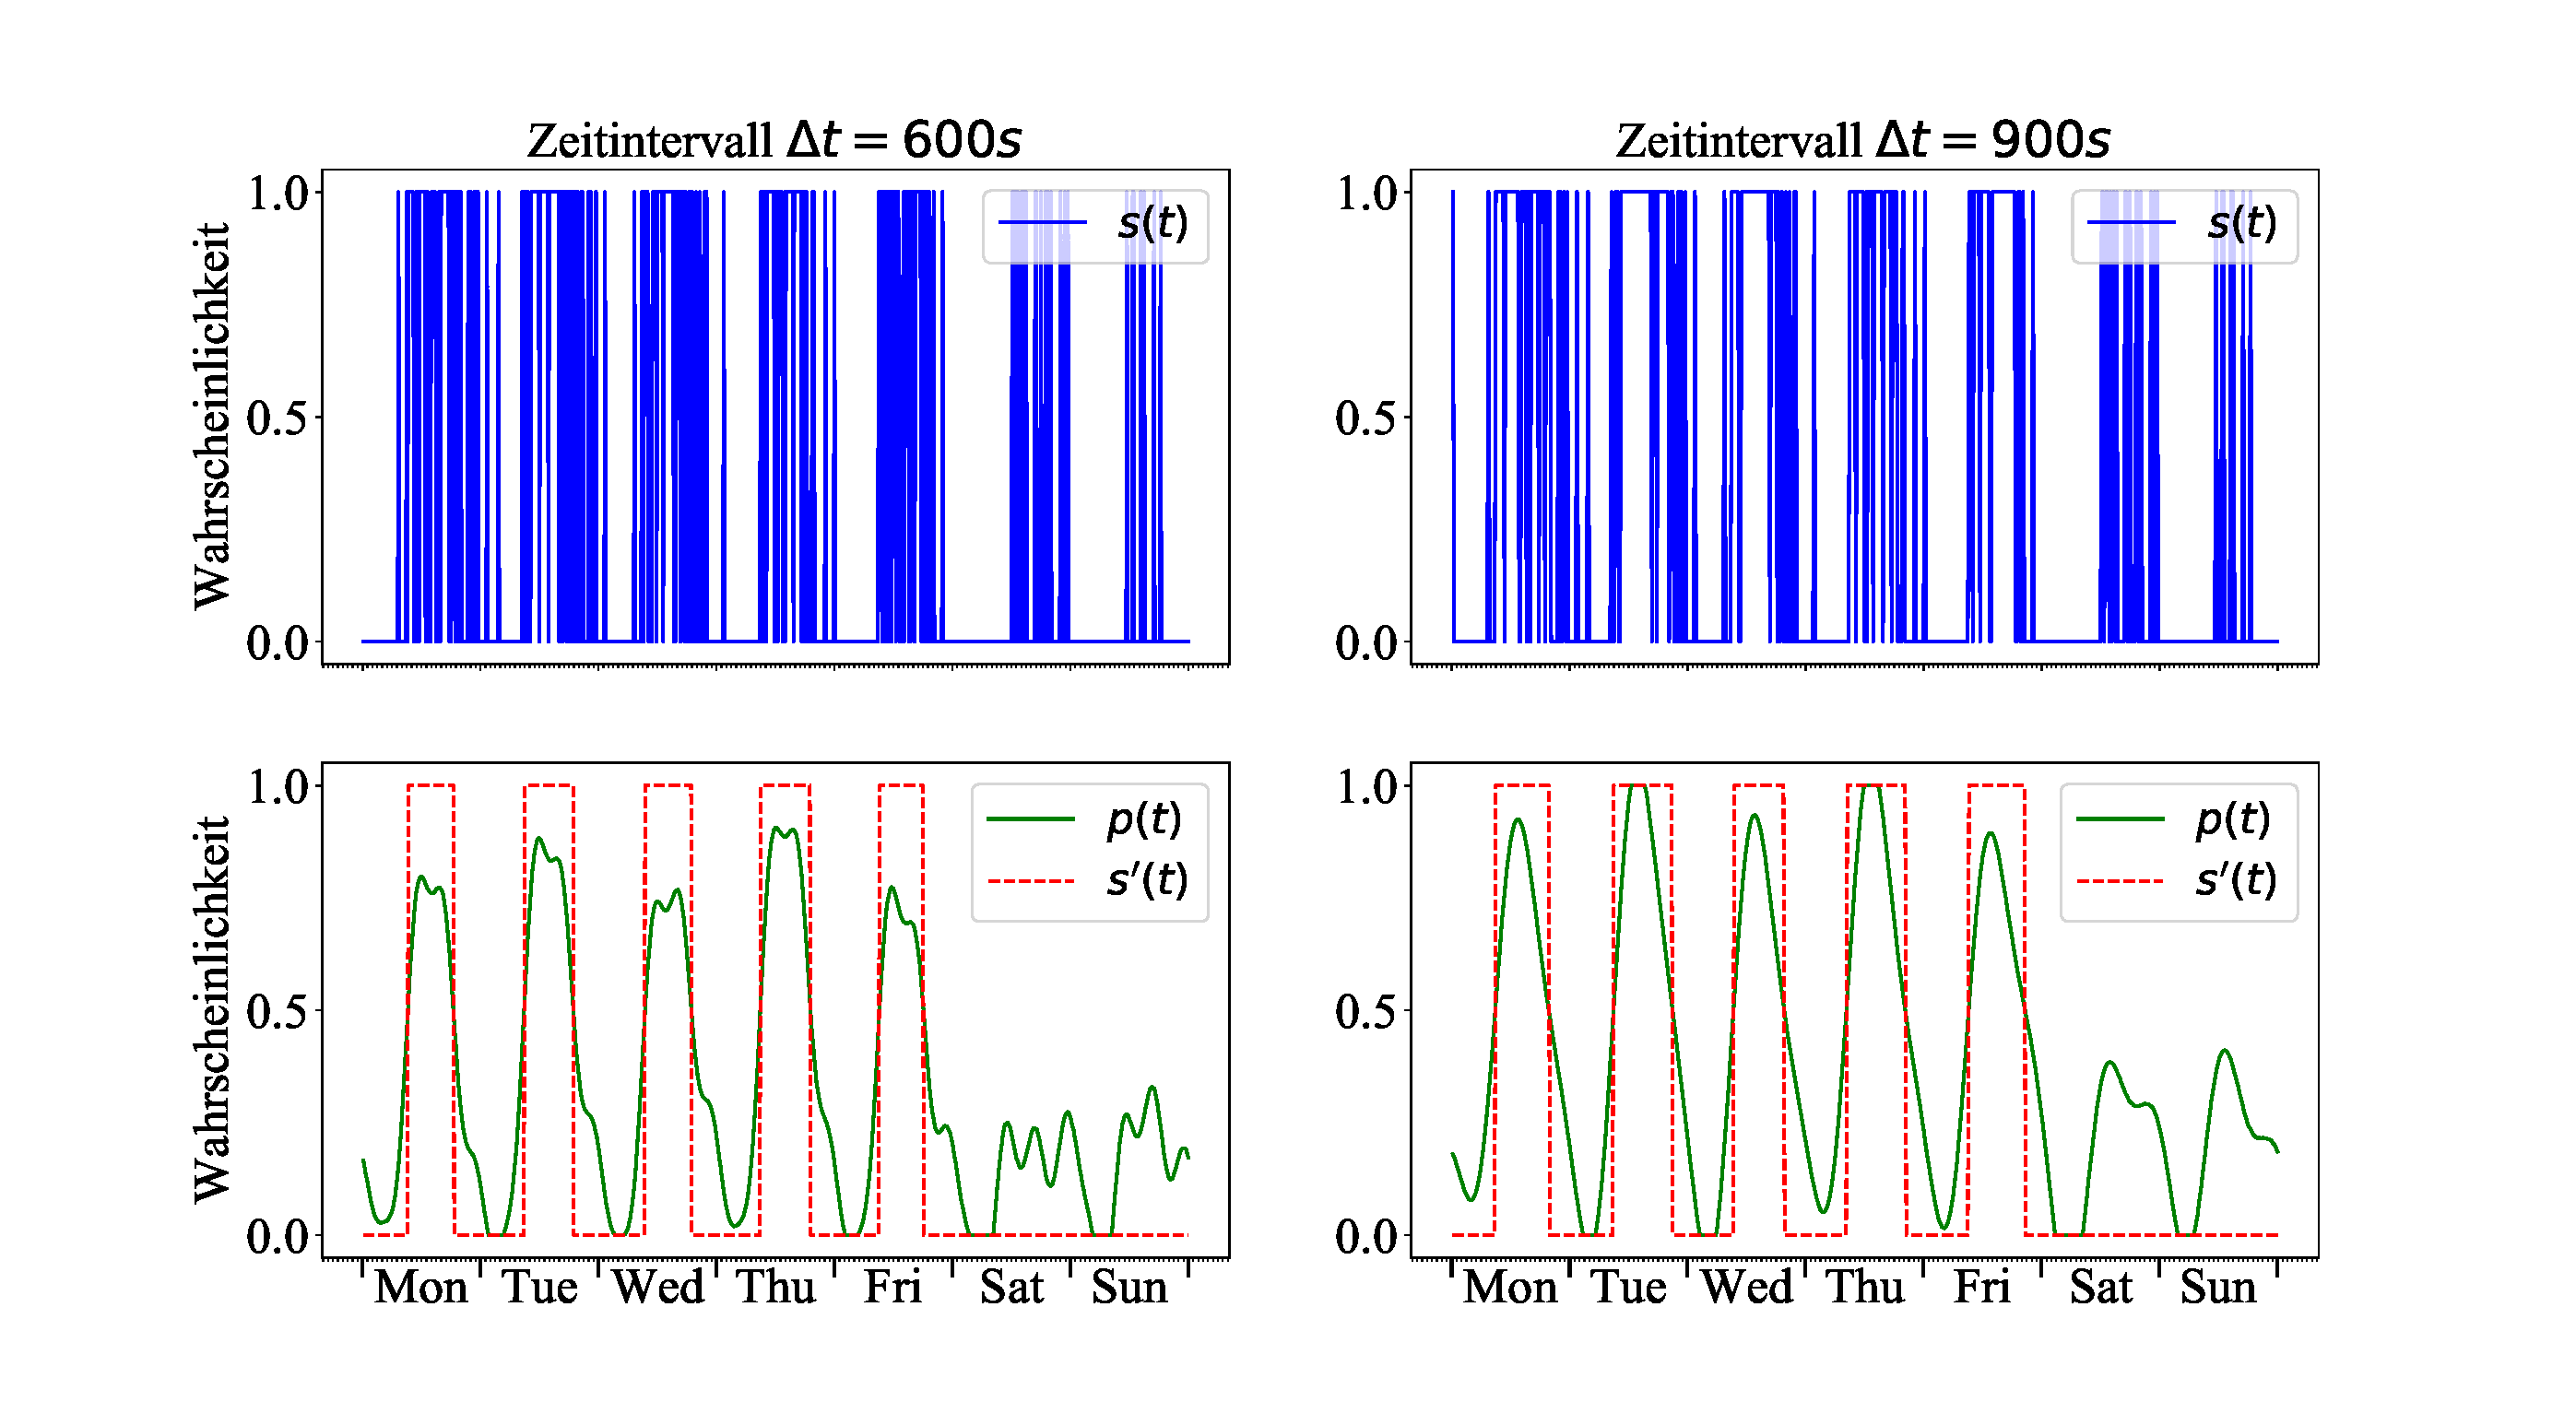
\includegraphics[width=1.0\linewidth]{Abbildungen/evaluation/bin_size_influence_cell_row_23_col_25_binary_numero_due}
	\caption{Zellzustand $s(t)$ sowie Wahrscheinlichkeitsfunktion $p(t)$ und prognostizierter Zellzustand $s'(t)$ einer Beispielzelle des UOL-Datensatzes mit einer Intervalldauer von $\Delta t = \SI{600}{\second} $ (links) und $\Delta t = \SI{900}{\second} $ (rechts)}
	\label{fig.bin_size_influence_cell_row_23_col_25_binary}
\end{figure}

Für die kürzere Intervalldauer $\Delta t = \SI{600}{\second}$ liegt die optimale Modellordnung bei $l_\ind{opt} = 10$ mit einem Prädiktionsfehler von $\epsilon_\ind{p,opt} = 15.1 \%$. Der Prädiktionsfehler des statischen Modells beträgt $\epsilon_\ind{p,stat} = 28.5 \%$. Es ist zu erkennen, dass das Modell den Wochentrend der Daten abbilden kann. An den beiden Wochenendtagen flachen die Amplituden der Wahrscheinlichkeitsfunktion des Zellzustandes $p(t)$ deutlich ab. Da sie den Schwellwert von $c = 0.5$ nicht überschreiten, liegt die Prädiktion des Zellzustandes während des Wochenendes bei $s'(t) = \mathrm{const}. = 0.0$. Bei einer Intervalldauer von $\Delta t = \SI{900}{\second} $ berechnet sich die optimale Modellordnung zu $l_\ind{opt} = 7$. Wie in \bild{bin_size_influence_master_bedroom_binary} resultiert eine Erhöhung der Intervalldauer $\Delta t$ in einer Vergrößerung der Breite der rot gestrichelten Balken der Prädiktion des Zellzustandes $s'(t)$. Erklären lässt sich dieses Verhalten damit, dass eine Verlängerung der Intervalldauer $\Delta t$ nach Gleichung \ref{eq:Number timestamps} zu einer Erhöhung des durchschnittlichen Zellzustandes $\bar{s}(t)$ führt. Auch das Modell der größeren Intervalldauer $\Delta t = \SI{900}{\second}$ kann den Wochentrend mit einem Abflachen der Personen-Auftrittswahrscheinlichkeiten während des Wochenendes abbilden. Liegt der Prädiktionsfehler der optimalen Modellordnung bei $\epsilon_\ind{p,opt} = 13.8 \%$, so beträgt er bei dem statischen Zustandsmodell $\epsilon_\ind{p,stat} = 35.3 \%$. \\
Einen zusammenfassenden Überblick der Modellfehler gibt Tabelle \ref{tab.Prädiktionsfehler uol_binary}.

\begin{table}[!h]
	\centering
	\caption{Prädiktionsfehler $\epsilon_\ind{p}$ bei unterschiedlichen Intervalldauern $\Delta t$ (UOL)}\label{tab.Prädiktionsfehler uol_binary}
	\vspace*{-3mm}
	\begin{tabular}{lcr}
		\toprule
		Intervalldauer $\Delta t$		& $\epsilon_\ind{p,opt}$	 & $\epsilon_\ind{p,stat}$          \\
		\midrule
		\SI{300}{\second}	& 8.93 \%         & 9.03 \%  \\
		\rowcolor{Snow2}
		\SI{600}{\second} 	& 10.49 \%        & 11.62 \% \\
		\SI{900}{\second}			& 10.75 \%      & 12.92 \% \\
		\bottomrule
	\end{tabular} 
\end{table}

% Auf Ergebnisse der Tabelle eingehen. Evtl letzte Spalte entfernen
% Betrachtet wurden nur Zellen, welche in mindestens fünf Prozent der Intervalle belegt % waren.

Aufgeteilt nach Intervalldauern sind hier die Prädiktionsfehler $\epsilon_\ind{p}$ aller Zellen für die optimale Modellordnung $l_\ind{opt}$ sowie für das statische Zustandsmodell aufgelistet. Es werden erneut nur die Zellen betrachtet, welche während mindestens 5 \% der betrachteten Zeitintervalle $\Delta t_i$ belegt waren. Diese Voraussetzung erfüllen nur 205 der insgesamt 3060 Zellen, in welche die Umgebung $\mathcal{U}$ eingeteilt wird.

Eine Darstellung des über die Umgebung $\mathcal{U}$ gelegten Gitters mit seinen einzelnen Zellen bietet \bild{original_binary_data}. Für ein beispielhaftes Zeitintervall $\Delta t_i$ mit einer Dauer von $\Delta t = \SI{600}{\second}$ ist hier für jede Zelle der zugehörige Zellstatus s(t) farblich dargestellt.



Zellen, welche innerhalb des Zeitintervalls belegt waren, sind in der Grafik rot markiert. Die restlichen, in blau eingefärbten Zellen, weisen während des entsprechenden Zeitintervalls keine Personendetektionen vor. Ein grafischer Vergleich zwischen den, mittels der optimalen Modellordnungen $l_\ind{opt}$ berechneten FreMEn-Modellen und den statischen Modellen der einzelnen Zellen kann mit Hilfe von \bild{binary_fremen_vs_static} gezogen werden.
\newpage
% caption ändern !
\begin{figure}[!ht]
	\centering
	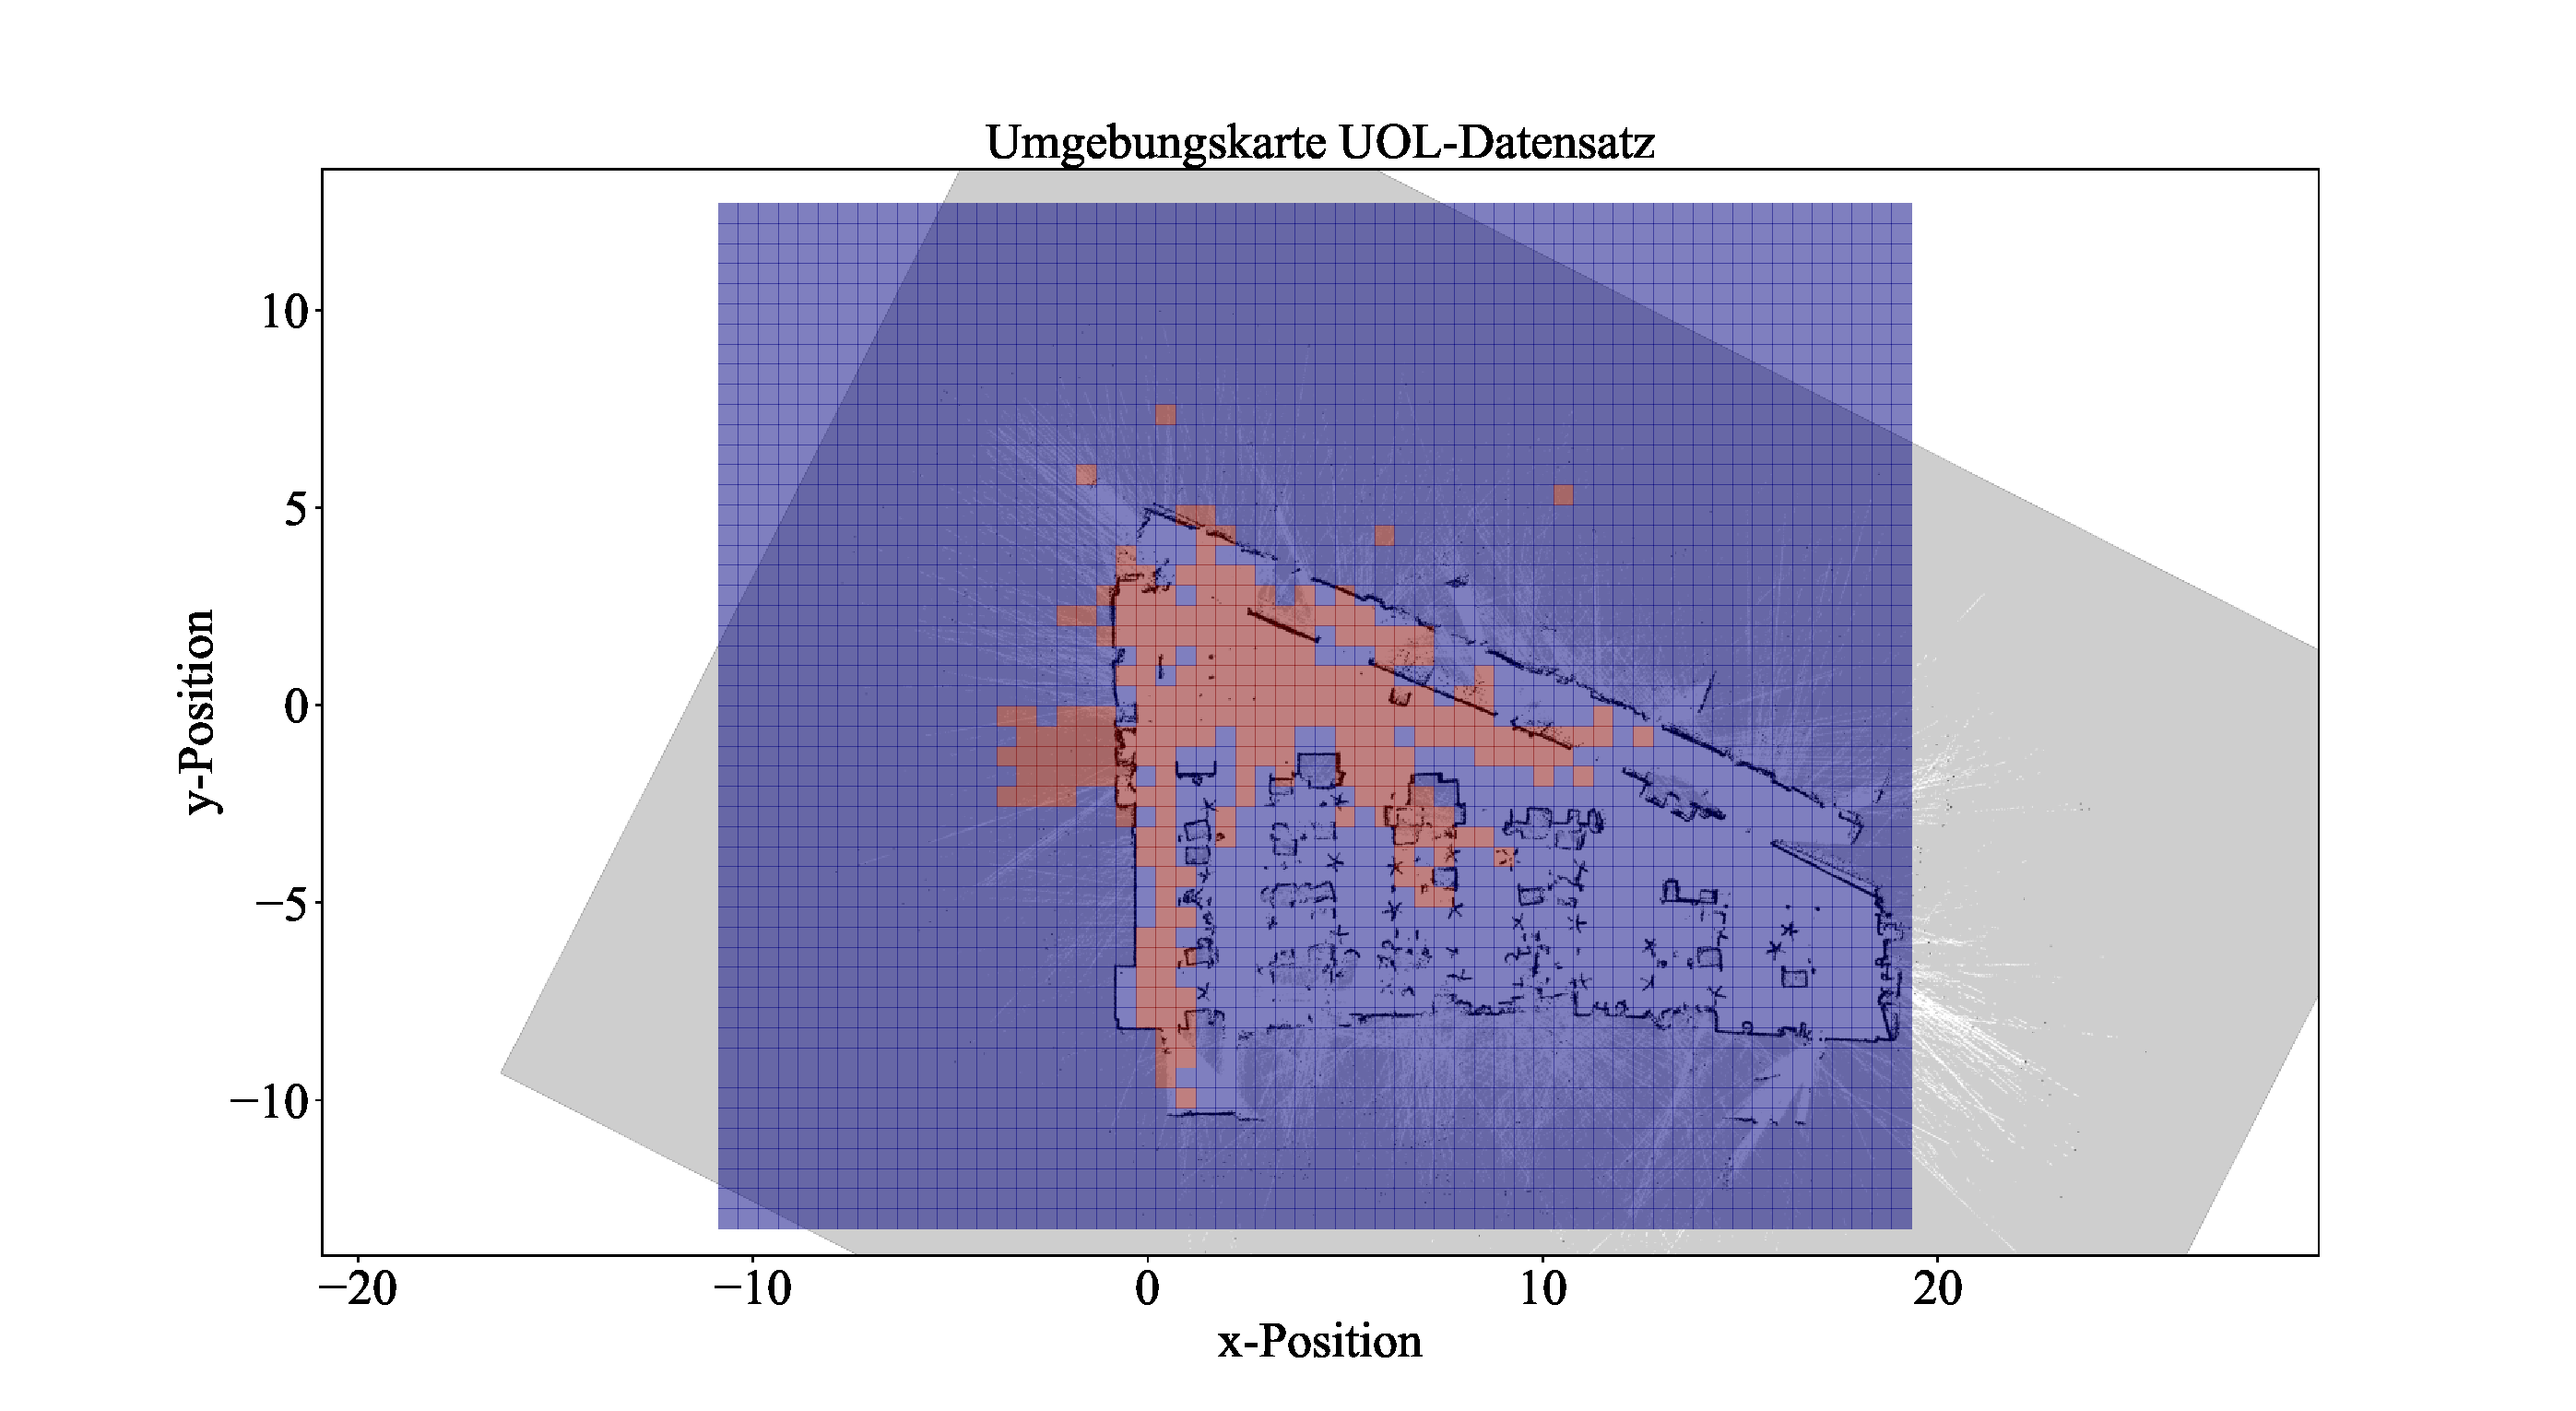
\includegraphics[width=1.0\linewidth]{Abbildungen/evaluation/original_binary_data}
	\caption{Tatsächliche Zellzustände s(t) des Belegungsgitters innerhalb eines beispielhaften Zeitintervalls $\Delta t_i$}
	\label{fig.original_binary_data}
\end{figure}
Zu erkennen ist, dass die FreMEn-Modelle (Bild \ref{fig.binary_best_prediction}) nur einen Teil der Gesamtheit der belegten Zellen als solche prognostizieren. Die als \textit{belegt} prognostizierten Zellen befinden sich allesamt innerhalb des Bürogebäudes. Die außerhalb des Gebäudes befindlichen, belegten Zellen (vlg. \bild{original_binary_data}) überschreiten im FreMEn-Modell nicht den Schwellwert von $c=0.5$ und werden somit als \textit{frei} prognostiziert. In Bild \ref{fig.binary_static} ist das statische Modell der einzelnen Zellen des Gitters dargestellt. Man erkennt, dass keine der Zellen innerhalb des betrachteten Zeitintervalls als \textit{belegt} prognostiziert worden ist. Die Begründung liegt darin, dass keine der einzelnen Zellen einen über den Gesamtzeitraum durchschnittlichen Zellzustand von $\bar{s(t)} = 0.5$ besitzt. Somit kann für keine Zelle der Schwellwert von $c=0.5$ überschritten werden. 

\begin{figure}[!h]
	\centering
	\subfigure[Prognostizierte Zellzustände s'(t) mit FreMen-Modellen der Ordnungen $l_\ind{opt}$\label{fig.binary_best_prediction}]{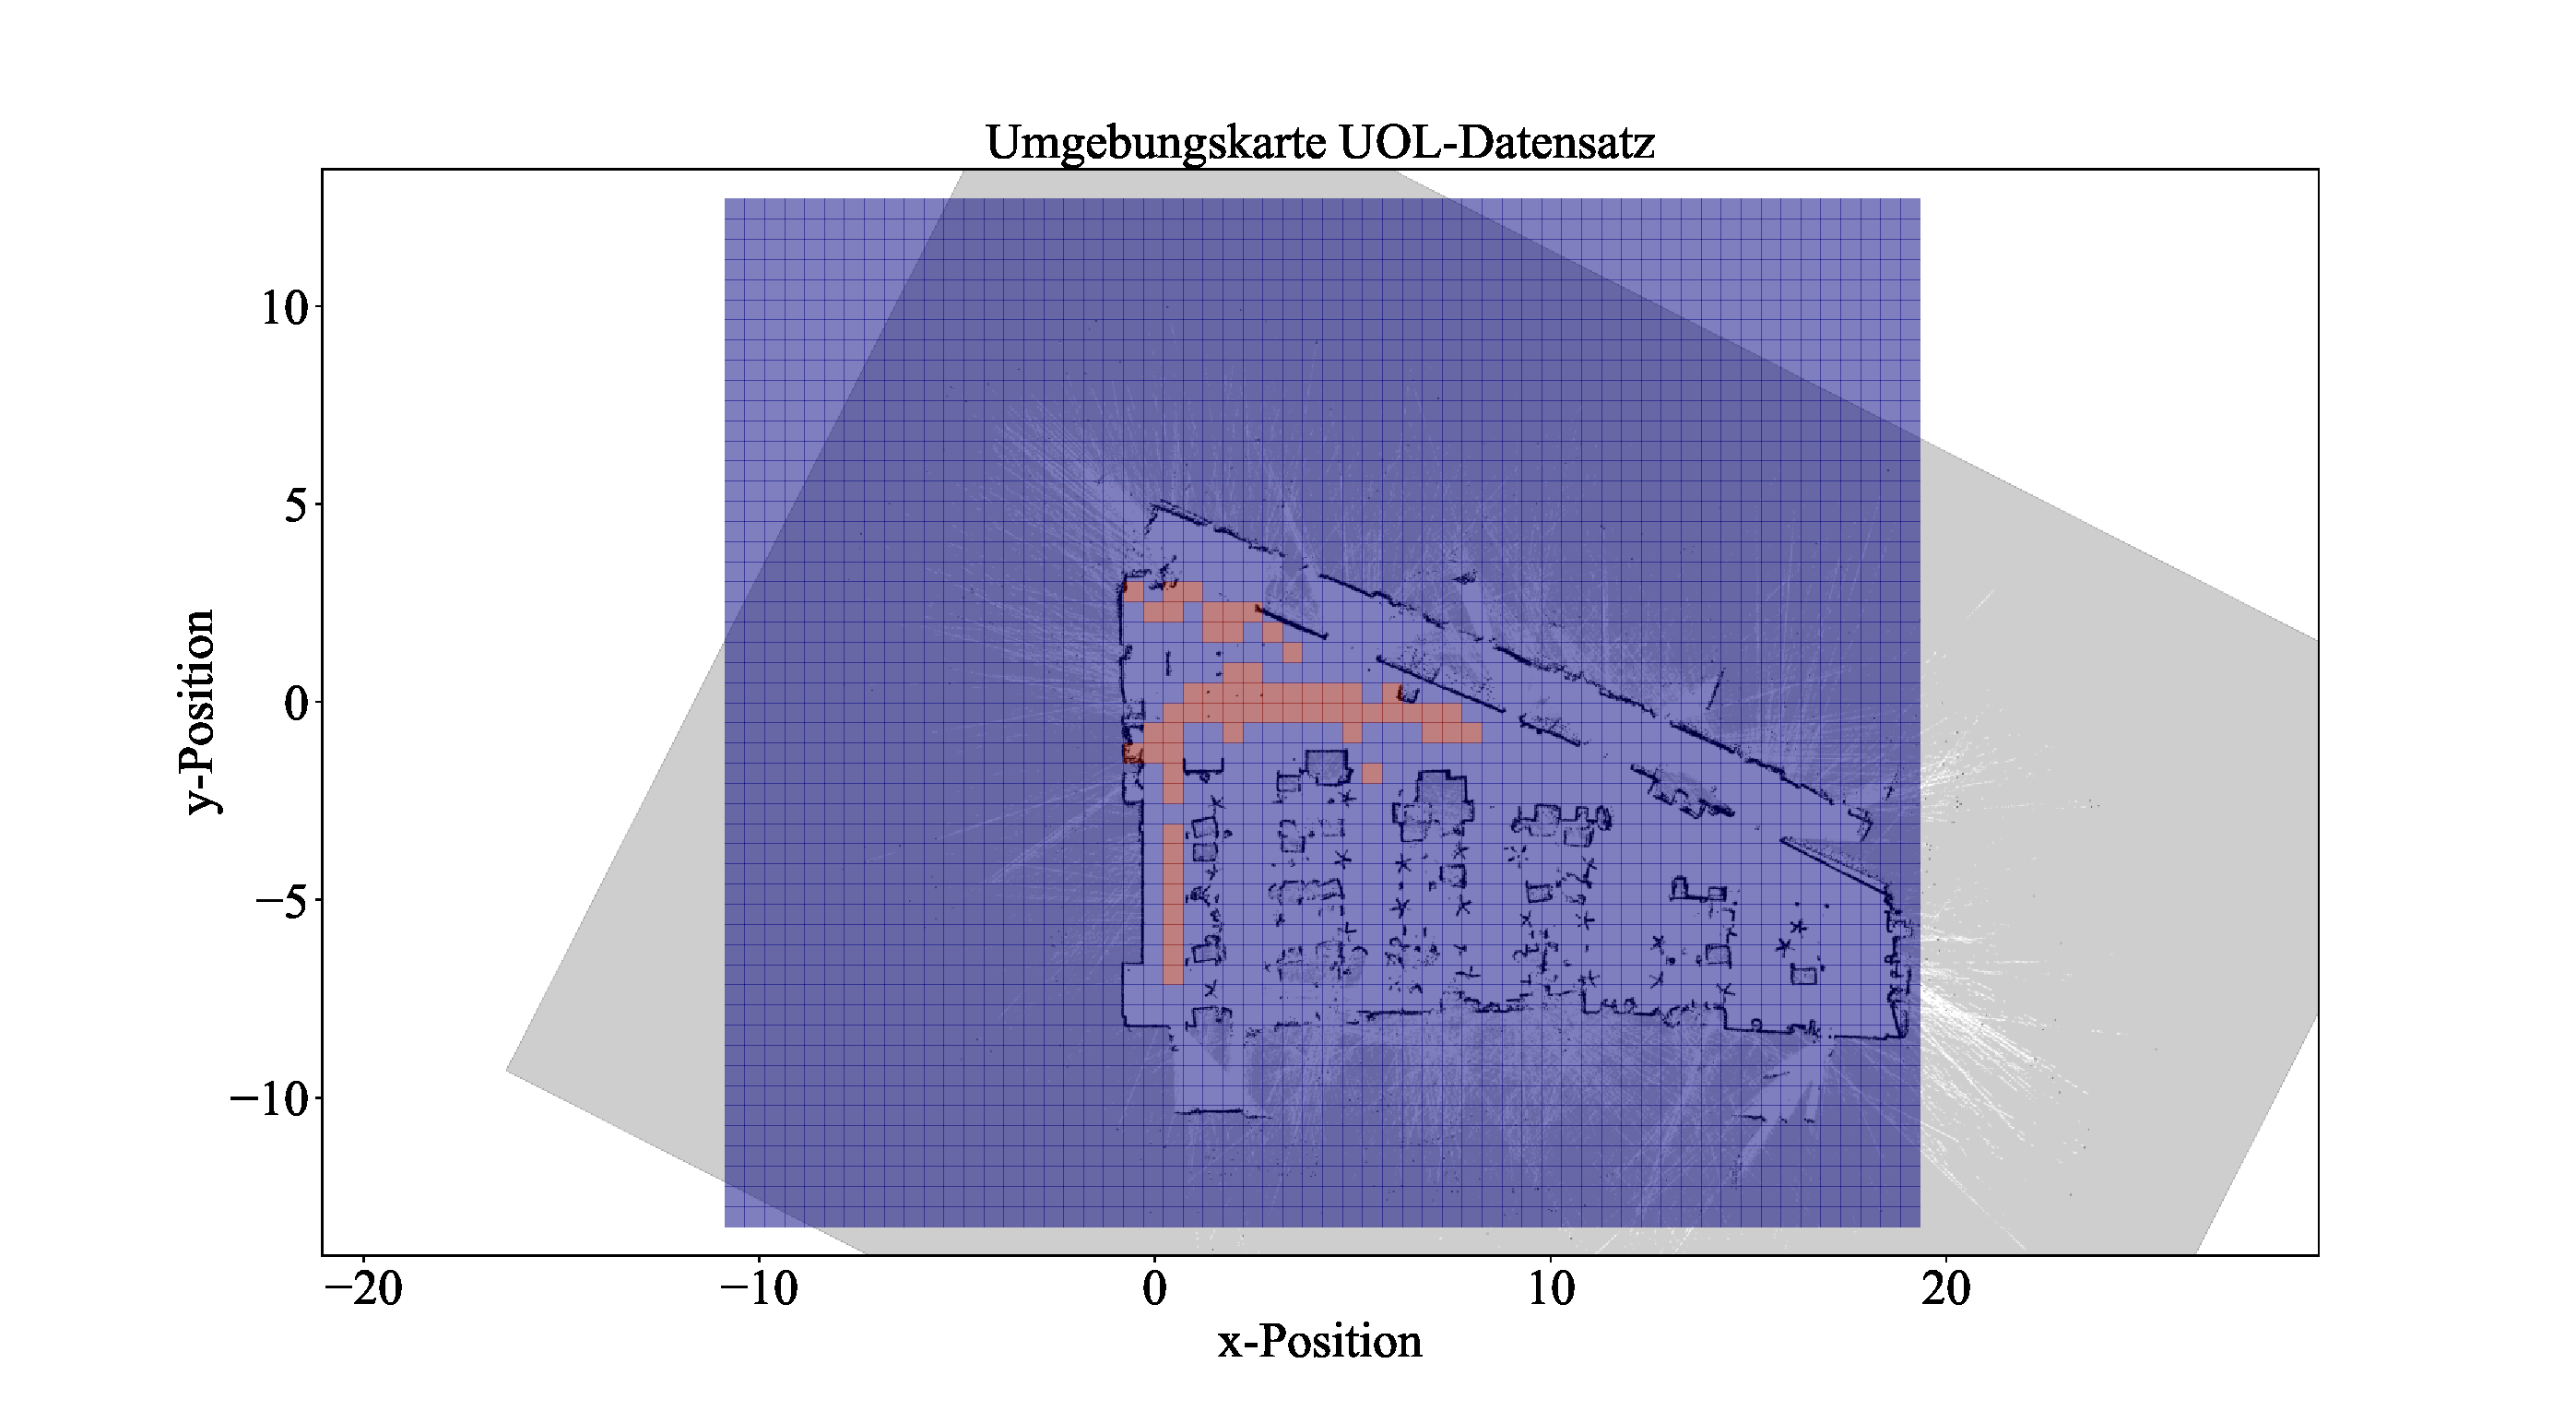
\includegraphics[width=1.0\linewidth]{Abbildungen/evaluation/binary_data_best_prediction}}

	\subfigure[Prognostizierte Zellzustände s'(t) mit statischen Modellen\label{fig.binary_static}]{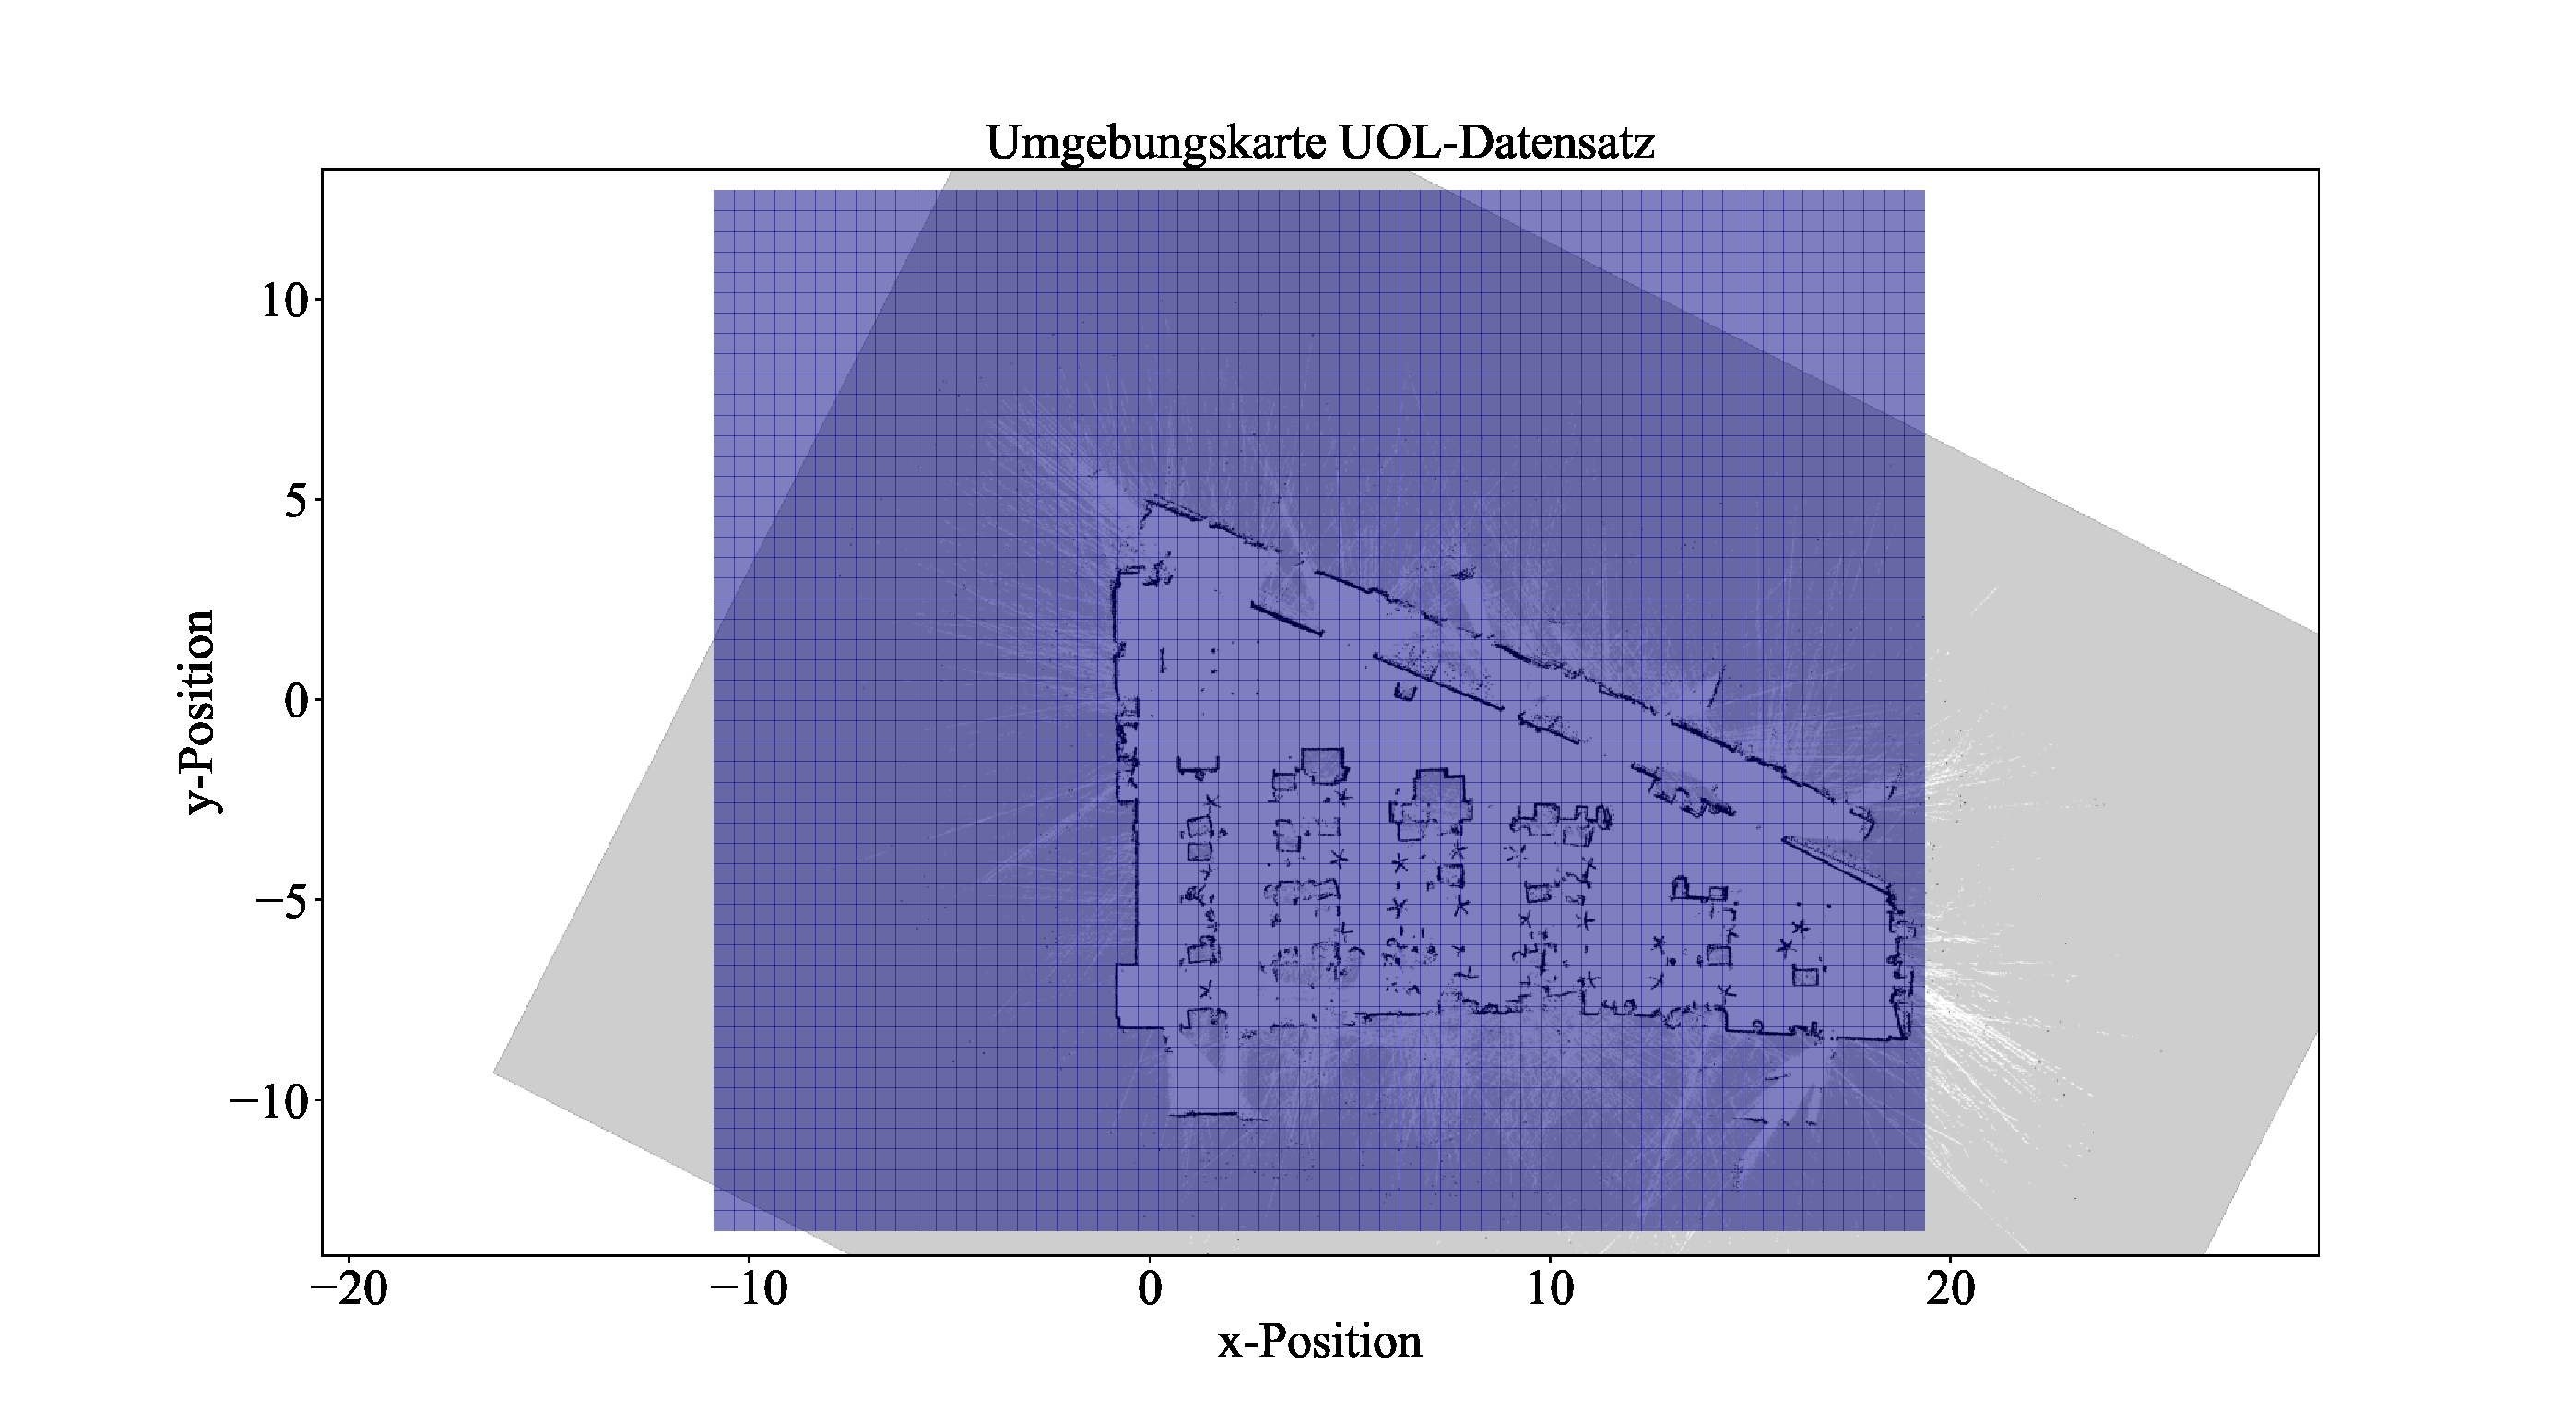
\includegraphics[width=1.0\linewidth]{Abbildungen/evaluation/binary_data_static}}
	\caption{Vergleich von FreMEn-Modellen mit statischen Modellen für den binären Fall}
	\label{fig.binary_fremen_vs_static}
\end{figure}



\newpage
\section{Quantitatives Modell}
\label{sec.Quantitatives Modell}

In diesem Abschnitt erfolgt eine Evaluation der quantitativen Modelle. Der betrachtete Wert ist die Personenrate $\lambda(t)$, also die Anzahl von Personen innerhalb eines Zeitintervalls. Veranschaulicht wird dies in \bild{bin_size_influence_master_bedroom_float_600}.

\begin{figure}[!h]
	\begin{center}
		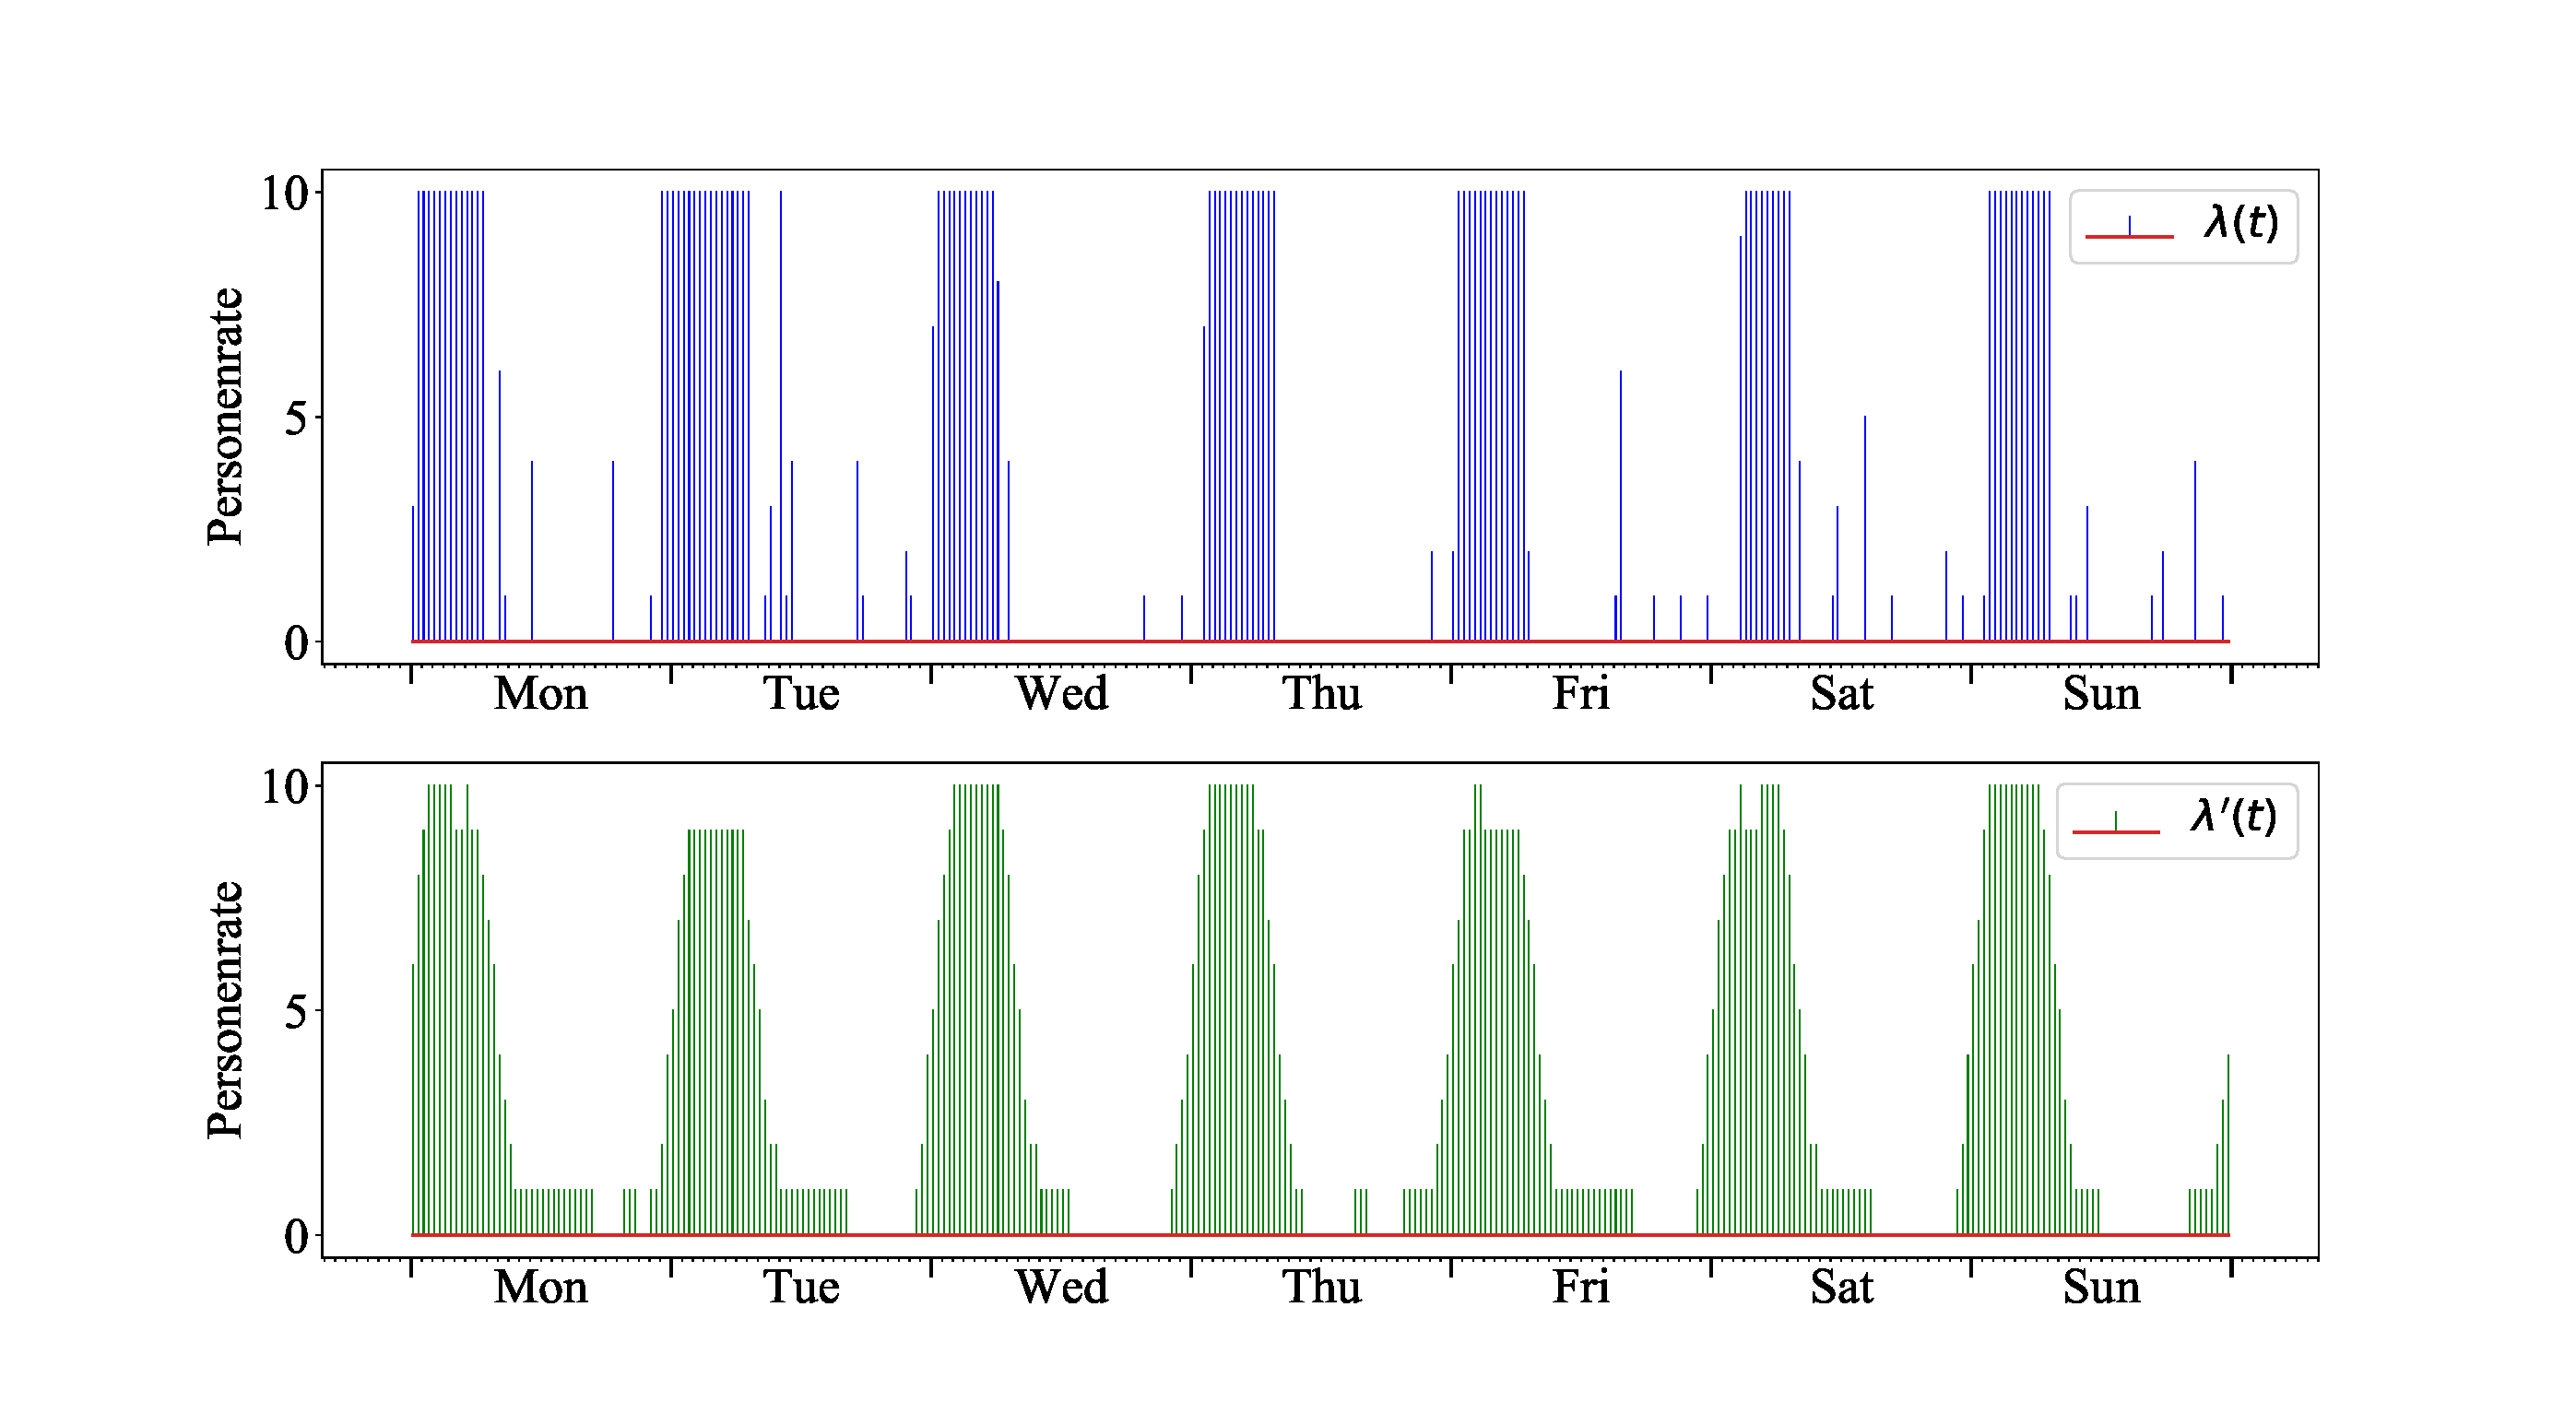
\includegraphics[width=\linewidth]{Abbildungen/evaluation/bin_size_influence_master_bedroom_float_600.pdf}
		\caption[Personenrate $\lambda (t)$  des Schlafzimmers (Aruba Datensatz) bei einer Intervalldauer von  $\Delta t = \SI{600}{\second}$ und Approximation $\lambda '(t)$]{Personenrate $\lambda (t)$  des Schlafzimmers (Aruba-Datensatz) bei einer Intervalldauer von  $\Delta t = \SI{600}{\second}$ (oben) und Approximation $\lambda '(t)$ (unten)}
		\label{fig.bin_size_influence_master_bedroom_float_600}
	\end{center}
\end{figure}

Dargestellt sind die Personenraten $\lambda (t)$ des Schlafzimmers des Aruba-Datensatzes  bei einer Intervalldauer von $\Delta t = \SI{600}{\second}$ (oben). Im Aruba-Datensatz wurde der Aufenthaltsort einer Person innerhalb der Räume der Wohnung minütlich dokumentiert. Die in \bild{bin_size_influence_master_bedroom_float_600} gewählte Intervalldauer resultiert also in einer maximalen Personenrate von $\lambda_\ind{max} = 10$. Im Bezug auf den Begriff \textit{Personenrate} sei angemerkt, dass sich diese im vorliegenden Zusammenhang lediglich auf dieselbe, innerhalb der Wohnung befindliche, Person bezieht.  Die optimale Modellordnung zur Berechnung von $\lambda '(t)$, also der Approximation der tatsächlichen Personenrate $\lambda(t)$, liegt bei $l_\ind{opt}=5$. Die Approximation ist in der unteren Grafik von \bild{bin_size_influence_master_bedroom_float_600} aufgezeichnet. Der Prädiktionsfehler  ergibt sich zu $\epsilon_\ind{p,opt} = 2.61$. Der Fehler wurde nach Gleichung \ref{eq:Prädiktionsfehler quantitativ} berechnet, die von dem Modell prognostizierte Personenrate $\lambda ' (t) $ hat also eine durchschnittliche Abweichung von 2.61 Personen pro Intervall von den tatsächlichen Daten. Die statische Personenrate beträgt $\lambda_\ind{stat} ' (t) = 4$. Der Prädiktionsfehler des statischen Modells liegt bei $\epsilon_\ind{p,stat} = 4.46$.
% In der oberen Grafik muss noch die statische Personenrate lambda_stat als gestrichelte gelbe Linie eingezeichnet werden.

\bild{bin_size_influence_master_bedroom_float_900} stellt $\lambda(t)$ bei einer Intervalldauer von $\Delta t = \SI{900}{\second}$ dar. Im Vergleich zu \bild{bin_size_influence_master_bedroom_float_600} liegen die Peaks von $\lambda (t)$ hier höher, was durch die größere Intervalldauer begründet ist. Die untere Grafik von \ref{fig.bin_size_influence_master_bedroom_float_900} stellt erneut die im Sinne von Gleichung \ref{eq:Prädiktionsfehler quantitativ} optimale Approximation $\lambda ' (t)$ von $\lambda (t)$ dar. Die optimale Modellordnung liegt erneut bei $l_\ind{opt} = 5$. Der Prädiktionsfehler liegt hier bei $\epsilon_\ind{p,opt} =  3.81$. Die Personenrate des statischen Modells lautet $\lambda_\ind{stat} ' = 5$. Der Prädiktionsfehler des statischen Modells beträgt $\epsilon_\ind{p,stat} = 6.62$. \\
Im Vergleich zum statischen Modell kann also mit einer Modellordnung von $l_\ind{opt} = 5$ eine Verbesserung um 43.45 \% erreicht werden.

\begin{figure}[!h]
	\begin{center}
		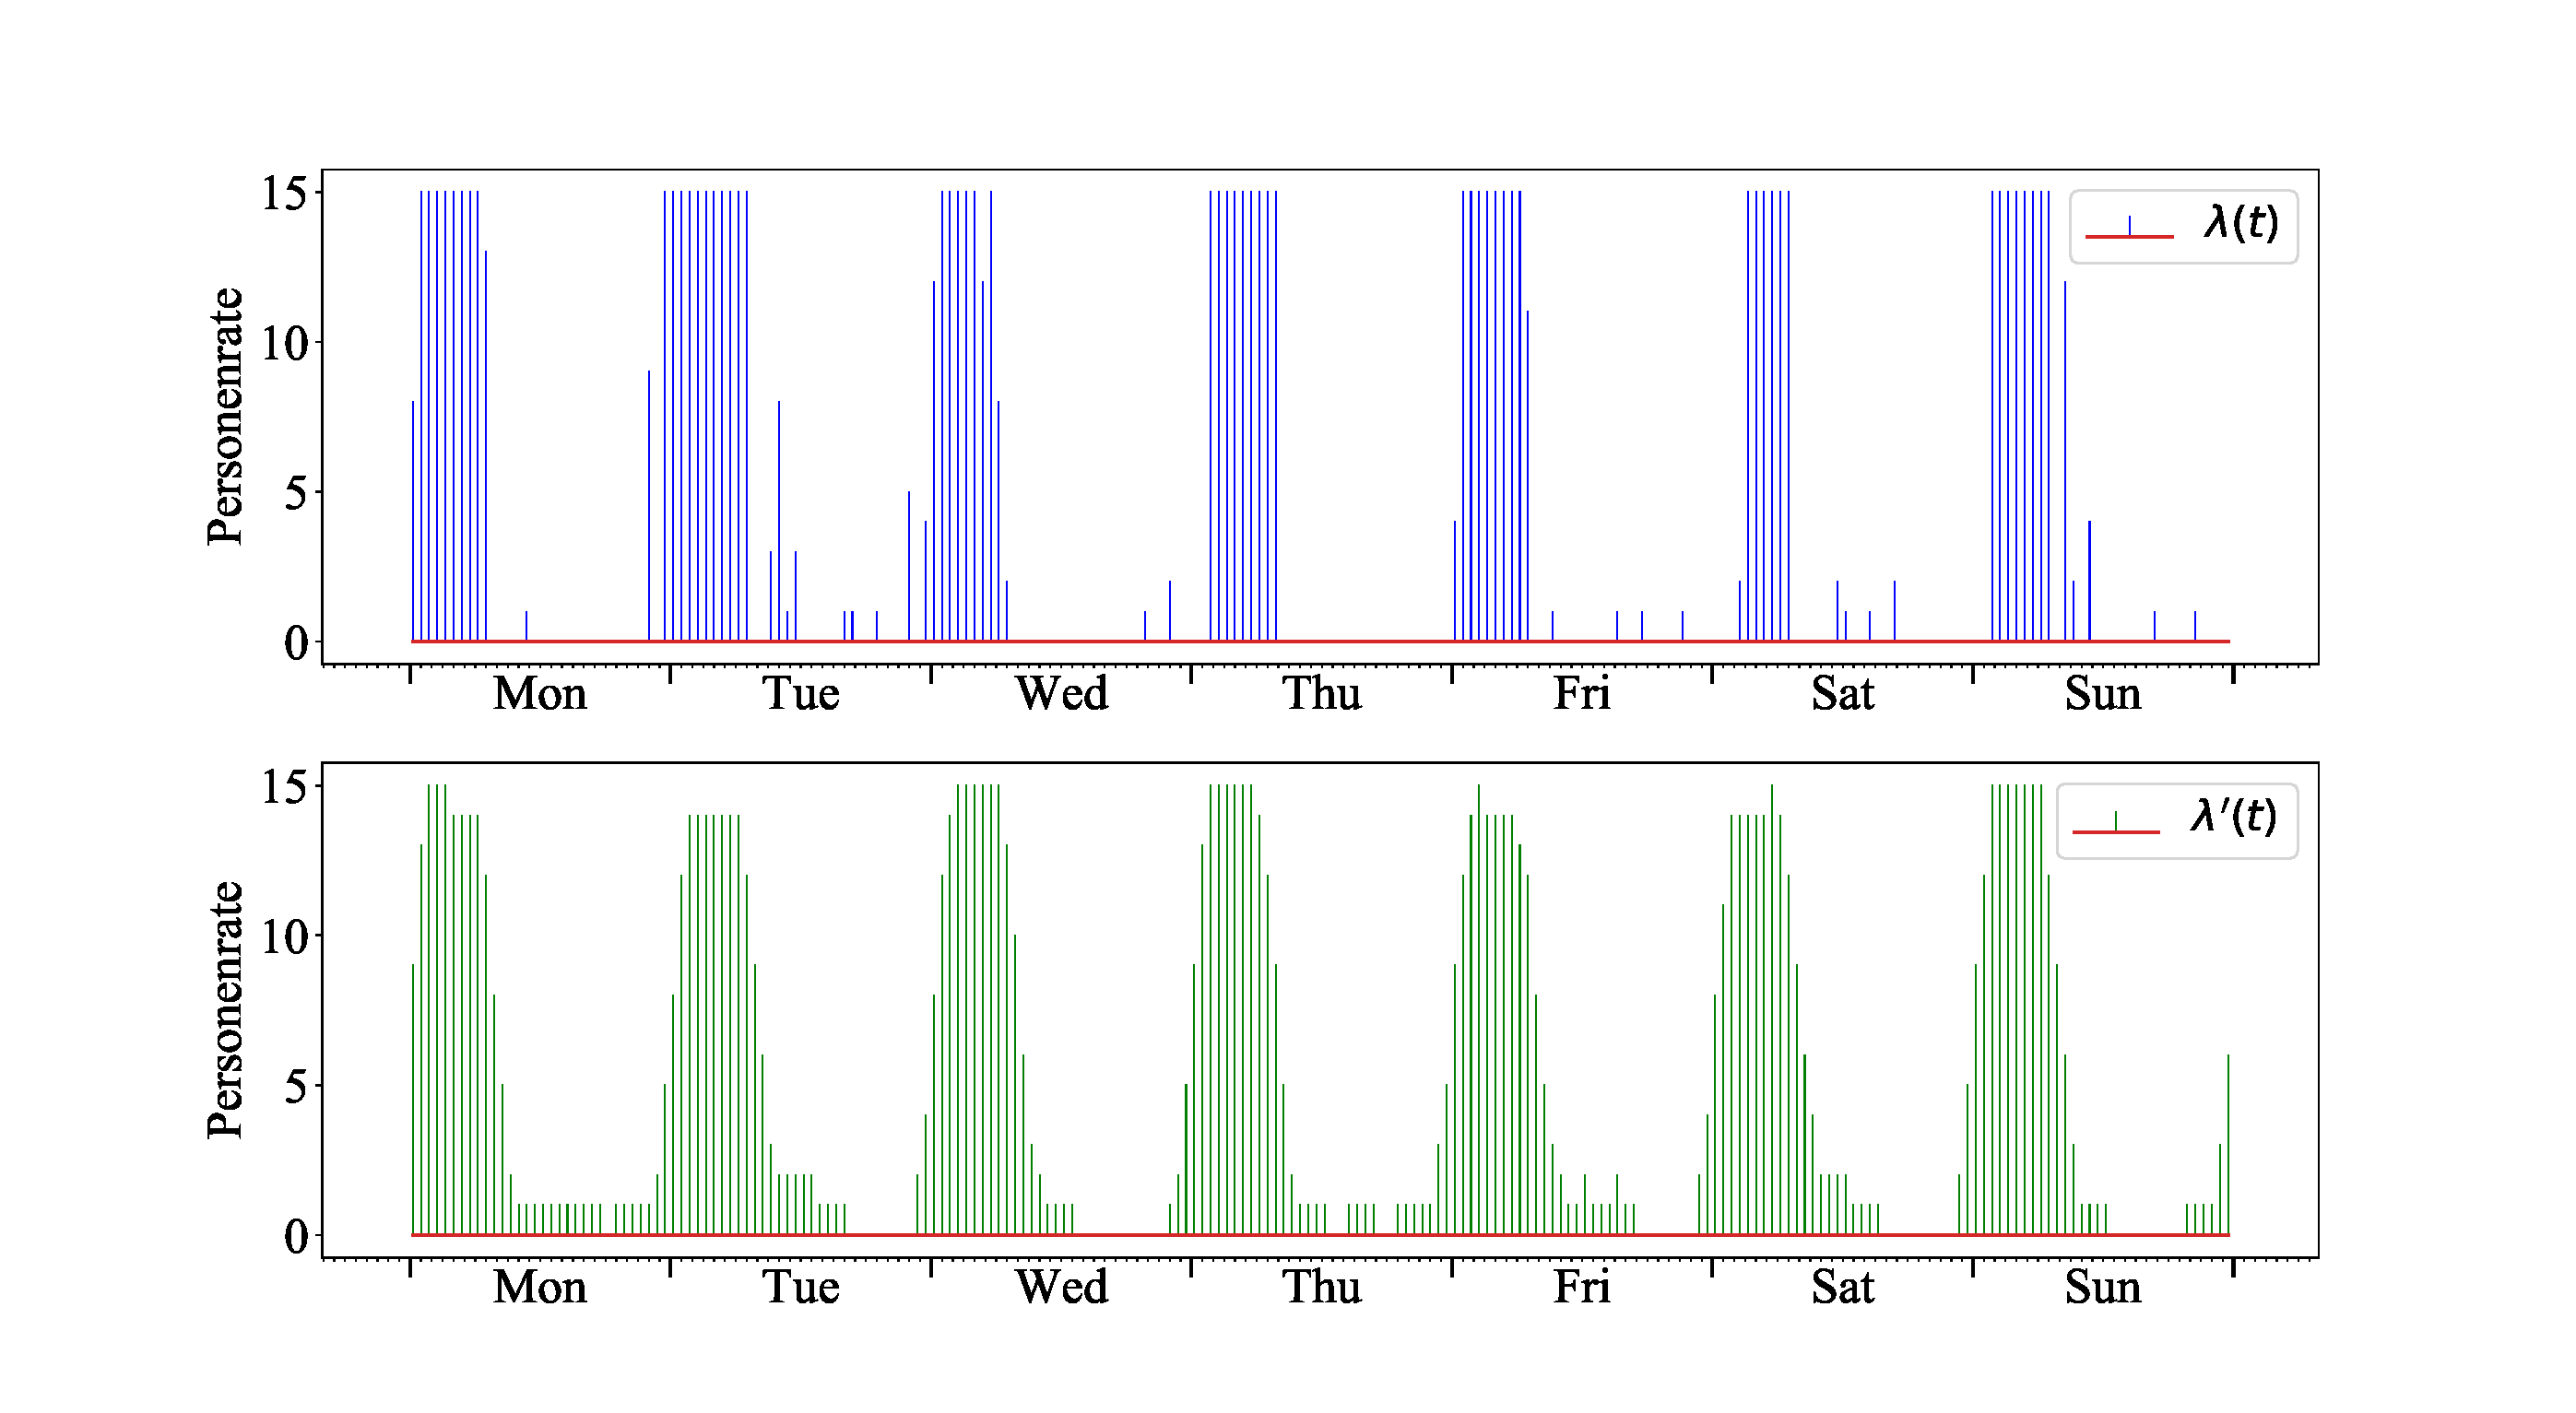
\includegraphics[width=\linewidth]{Abbildungen/evaluation/bin_size_influence_master_bedroom_float_900.pdf}
		\caption[Personenrate $\lambda (t)$ des Schlafzimmers bei einer Intervalldauer von  $\Delta t = \SI{600}{\second}$ und Approximation $\lambda '(t)$]{Personenrate $\lambda (t)$ des Schlafzimmers (Aruba-Datensatz) bei einer Intervalldauer von  $\Delta t = \SI{600}{\second}$ (oben) und Approximation $\lambda '(t)$ (unten)}
		\label{fig.bin_size_influence_master_bedroom_float_900}
	\end{center}
\end{figure}

Die Personenraten $\lambda(t)$ des Gästeschlafzimmers mit einer Intervalldauer von $\Delta t = \SI{600}{\second}$ sind in \bild{bin_size_influence_second_bedroom_float_600.pdf} aufgezeichnet. Die beste Approximation $\lambda ' (t)$ wird hierbei mit einer Ordnung von $l_\ind{opt} = 0$, also dem statischen Modell, erreicht. Die Prädiktion lautet für alle Intervalle $\lambda_\ind{stat} ' (t) = 0$. Der Prädiktionsfehler  beträgt $\epsilon_\ind{p} = 1.39$. 

\begin{figure}[!h]
	\begin{center}
		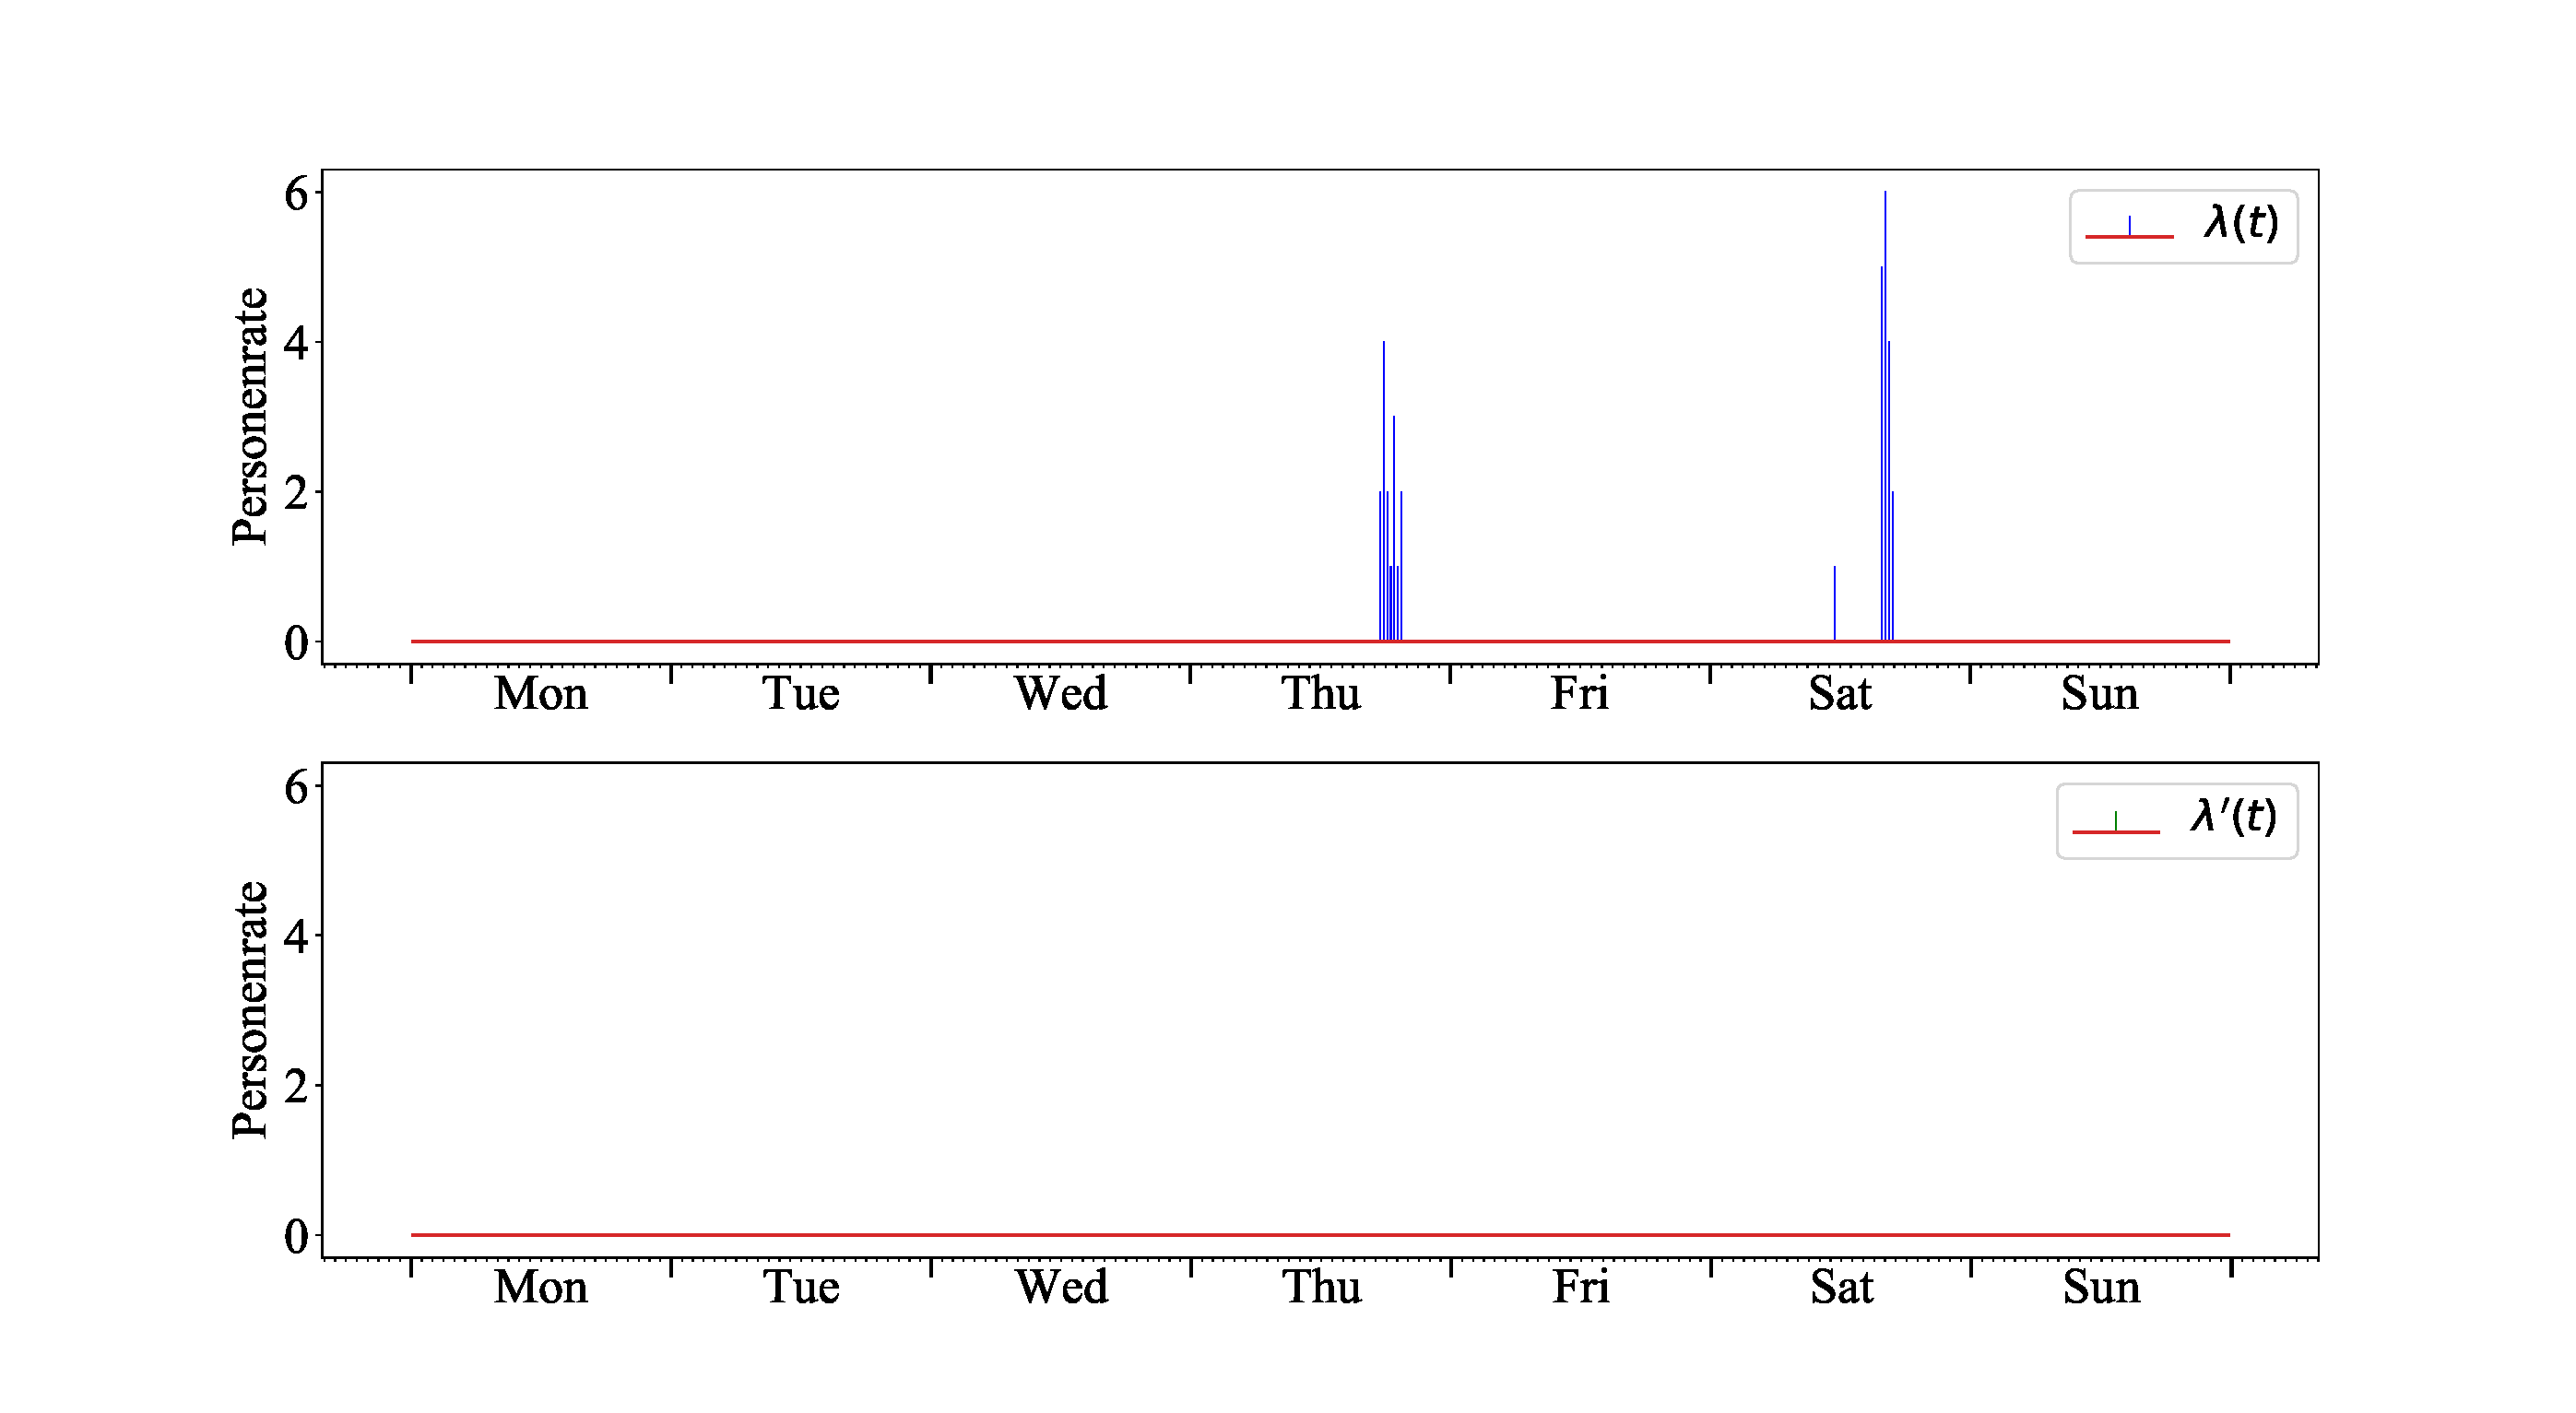
\includegraphics[width=\linewidth]{Abbildungen/evaluation/bin_size_influence_second_bedroom_float_600.pdf}
		\caption[Personenrate $\lambda (t)$ des Gästeschlafzimmers bei einer Intervalldauer von  $\Delta t = \SI{600}{\second}$ und Approximation $\lambda '(t)$]{Personenrate $\lambda (t)$ des Gästeschlafzimmers (Aruba-Datensatz) bei einer Intervalldauer von  $\Delta t = \SI{600}{\second}$ (oben) und Approximation $\lambda '(t)$ (unten)}
		\label{fig.bin_size_influence_second_bedroom_float_600.pdf}
	\end{center}
\end{figure}

Die untere Grafik von \bild{bin_size_influence_second_bedroom_float_900.pdf} veranschaulicht $\lambda (t)$ bei einer Intervalldauer von $\Delta t = \SI{900}{\second}$. Die beste Approximation wird in diesem Fall ebenfalls mit einer Modellordnung von $l_\ind{opt}=0$, also dem statischen Modell mit $\lambda_\ind{stat} ' (t) = \mathrm{const}.$ , erreicht. Die Prädiktion lautet nun für alle Intervalle $\lambda_\ind{stat} '(t) = 1$. Dies ist dadurch zu begründen, dass die durchschnittliche Personenrate bei größerer Intervalldauer steigt, und somit im Gegensatz zu \bild{bin_size_influence_second_bedroom_float_600.pdf} auf die nach Gleichung \ref{eq:Personenraten-Funktion} nächstgelegene natürliche Zahl gerundet wird, welche in diesem Fall 1 beträgt.

\begin{figure}[!h]
	\begin{center}
		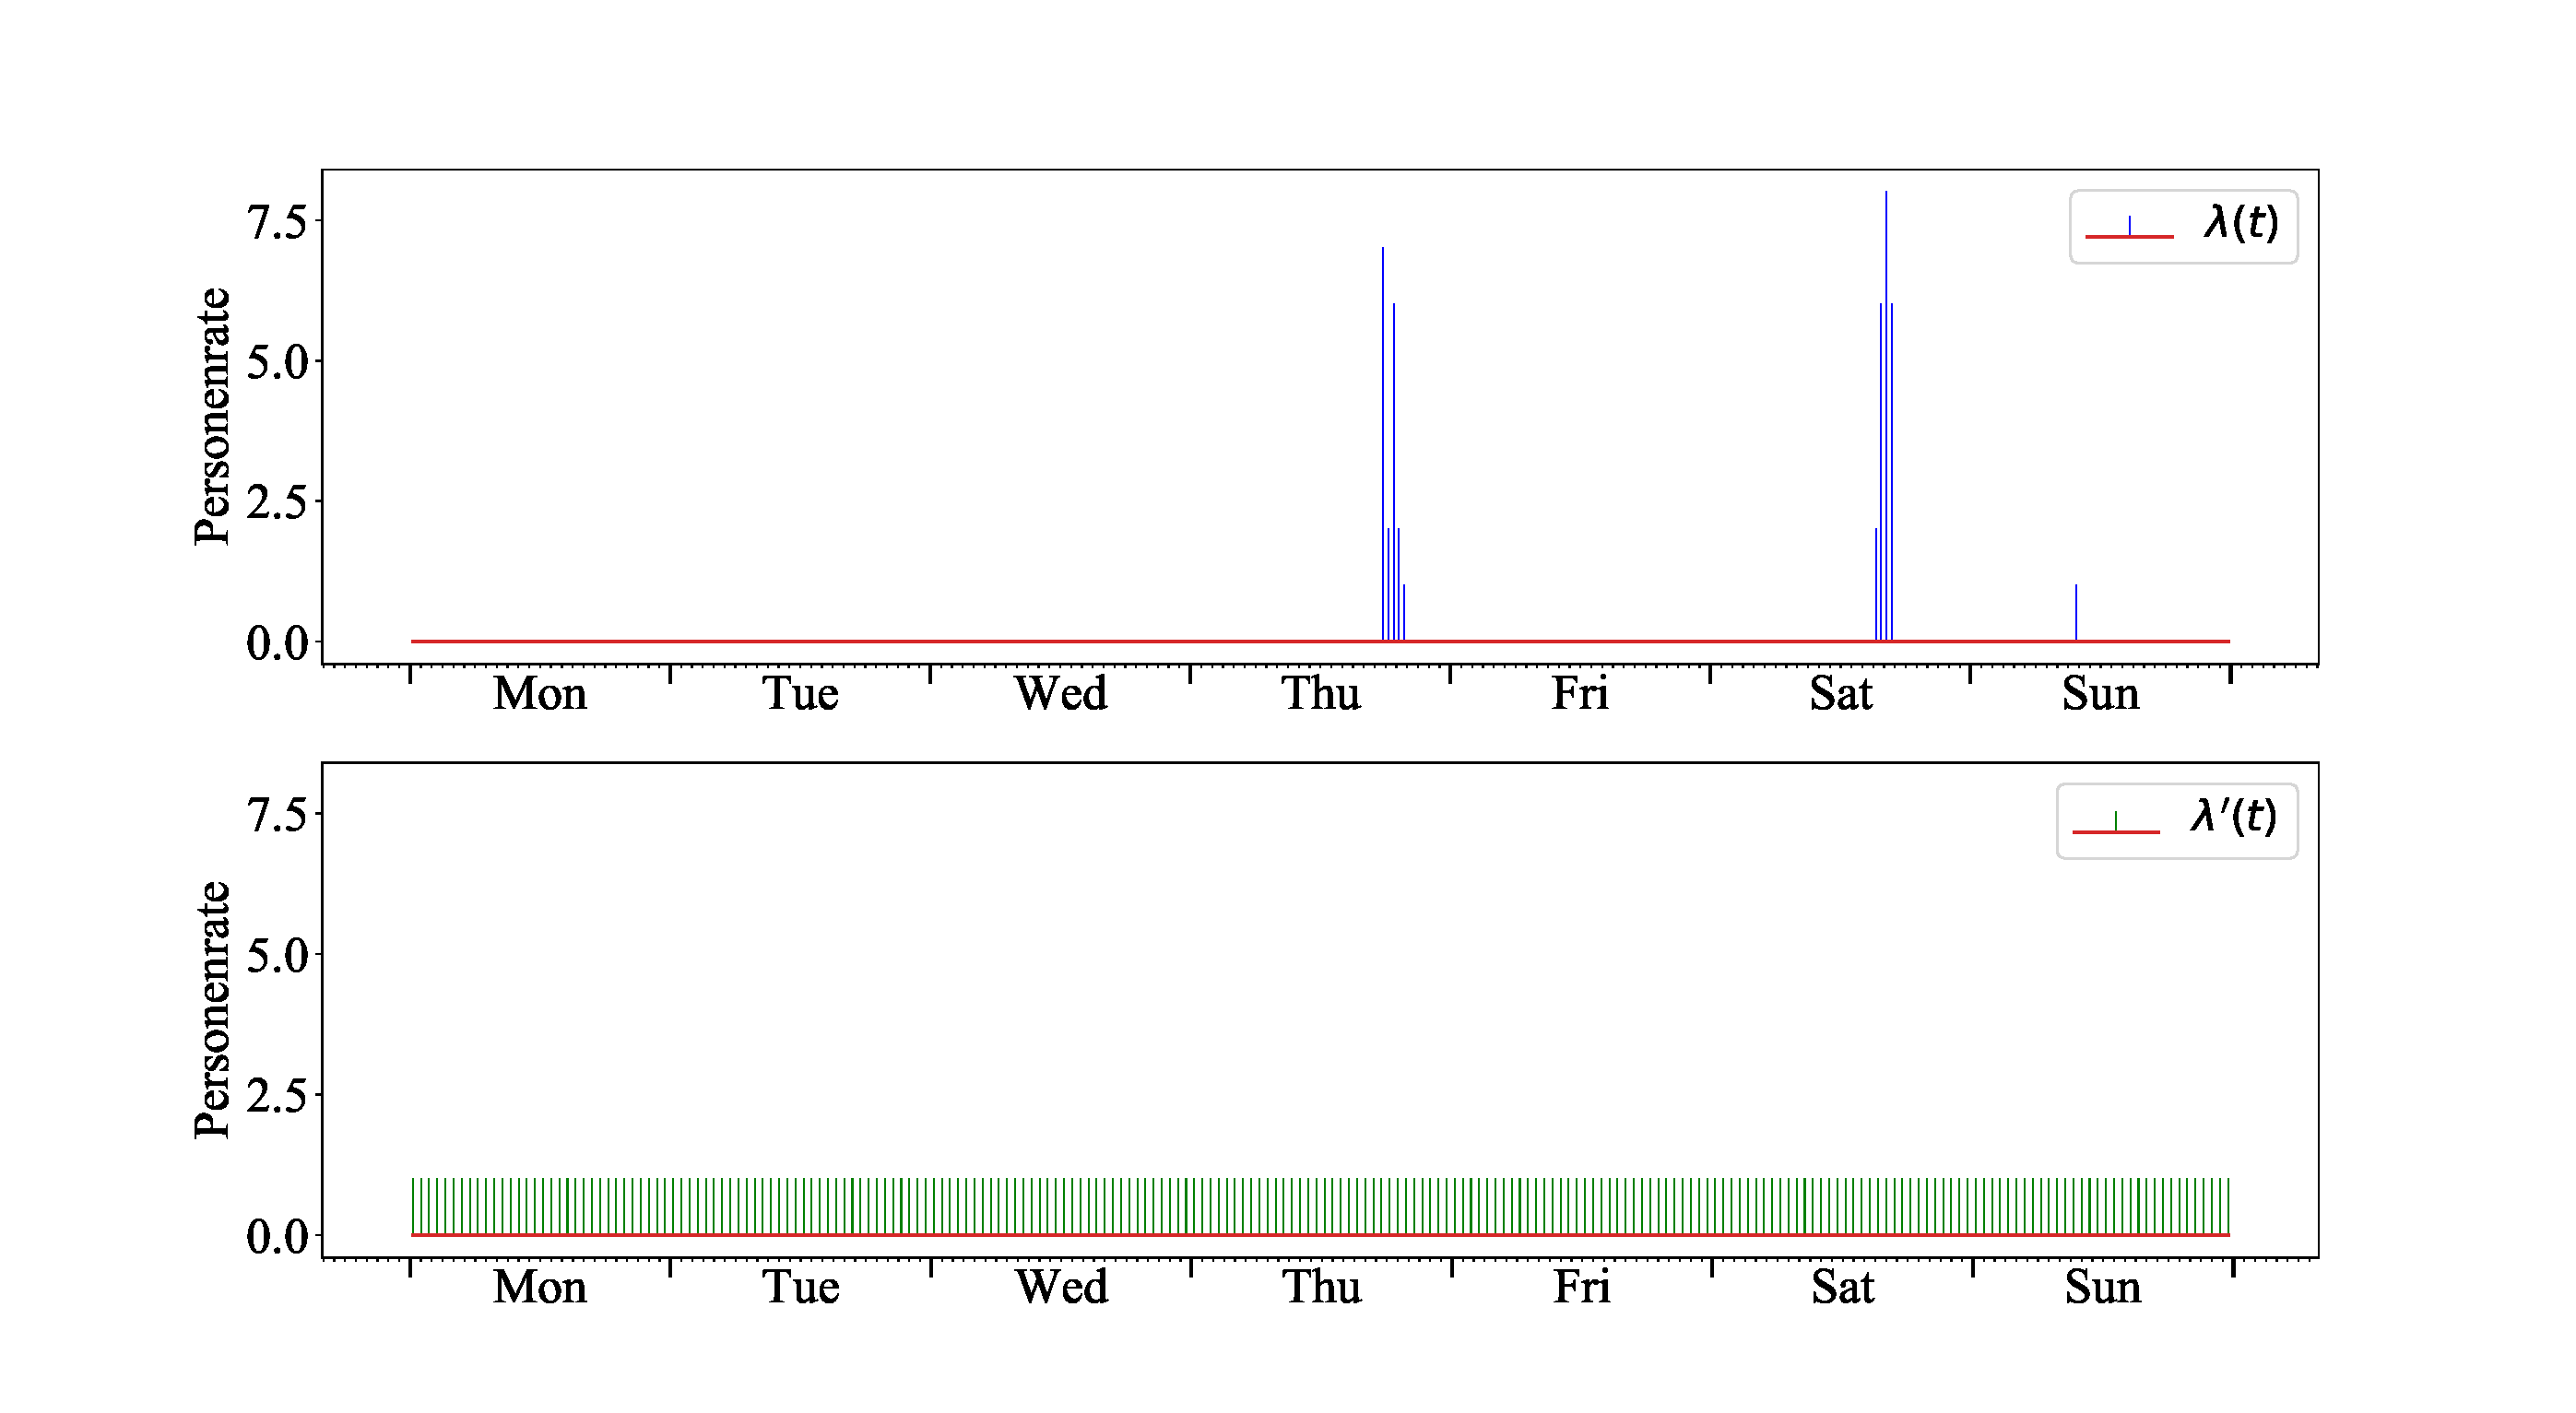
\includegraphics[width=\linewidth]{Abbildungen/evaluation/bin_size_influence_second_bedroom_float_900.pdf}
		\caption[Personenrate $\lambda (t)$ des Gästeschlafzimmers bei einer Intervalldauer von  $\Delta t = \SI{600}{\second}$ und Approximation $\lambda '(t)$]{Personenrate $\lambda (t)$ des Gästeschlafzimmers (Aruba-Datensatz) bei einer Intervalldauer von  $\Delta t = \SI{600}{\second}$ (oben) und Approximation $\lambda '(t)$ (unten)}
		\label{fig.bin_size_influence_second_bedroom_float_900.pdf}
	\end{center}
\end{figure}

Der Prädiktionsfehler  ergibt sich zu $\epsilon_\ind{p} = 2.04$. In Tabelle \ref{tab.Prädiktionsfehler aruba_float} sind die durchschnittlichen Prädiktionsfehler der Zellen des Datensatzes bei verschiedenen Intervalldauern aufgeführt. In die Fehlerermittlung flossen nur solche Zellen ein, bei denen in mindestens 5 \% der Intervalle eine Person detektiert worden ist. Unter Berücksichtigung dieser Voraussetzung wurden sieben der insgesamt zehn Räume bzw. Zellen des Aruba-Datensatzes zur Fehlerermittlung in Tabelle \ref{tab.Prädiktionsfehler aruba_float} genutzt.

\begin{table}[!h]
	\centering
	\caption{Prädiktionsfehler $\epsilon_\ind{p}$ bei unterschiedlichen Intervalldauern $\Delta t$ (Aruba)} \label{tab.Prädiktionsfehler aruba_float}
	\vspace*{-3mm}
	\begin{tabular}{lccr}
		\toprule
		Intervalldauer $\Delta t$		& $\epsilon_\ind{p,opt}$ & $\epsilon_\ind{p,stat}$  & Vergleich $\epsilon_\ind{p,opt}$ zu $\epsilon_\ind{p,stat}$              \\
		\midrule
		\SI{300}{\second}	& 1.17        & 1.43 & -18.18 \% \\
		\rowcolor{Snow2}
		\SI{600}{\second} 	& 2.23       & 2.76 & -19.20 \% \\
		\SI{900}{\second}			& 2.81        & 3.51 & -19.94 \% \\
		\bottomrule
	\end{tabular} 
\end{table}

Eine weitere Evaluation des Modells erfolgt anhand des UOL-Datensatzes. \bild{bin_size_influence_cell_row_23_col_25_float_600} zeigt die Personenraten $\lambda (t)$ bei einer Intervalldauer von $\Delta t = \SI{600}{\second}$ sowie die Prädiktion $\lambda ' (t) $ der optimalen Modellordnung $l_\ind{opt} = 2$ mit einem Prädiktionsfehler von $\epsilon_\ind{p,opt} = 11.38$.
% Hier Abbildung bin_size_influence_cell_row_23_col_25_float_600.pdf einfügen
\begin{figure}[!h]
	\centering
	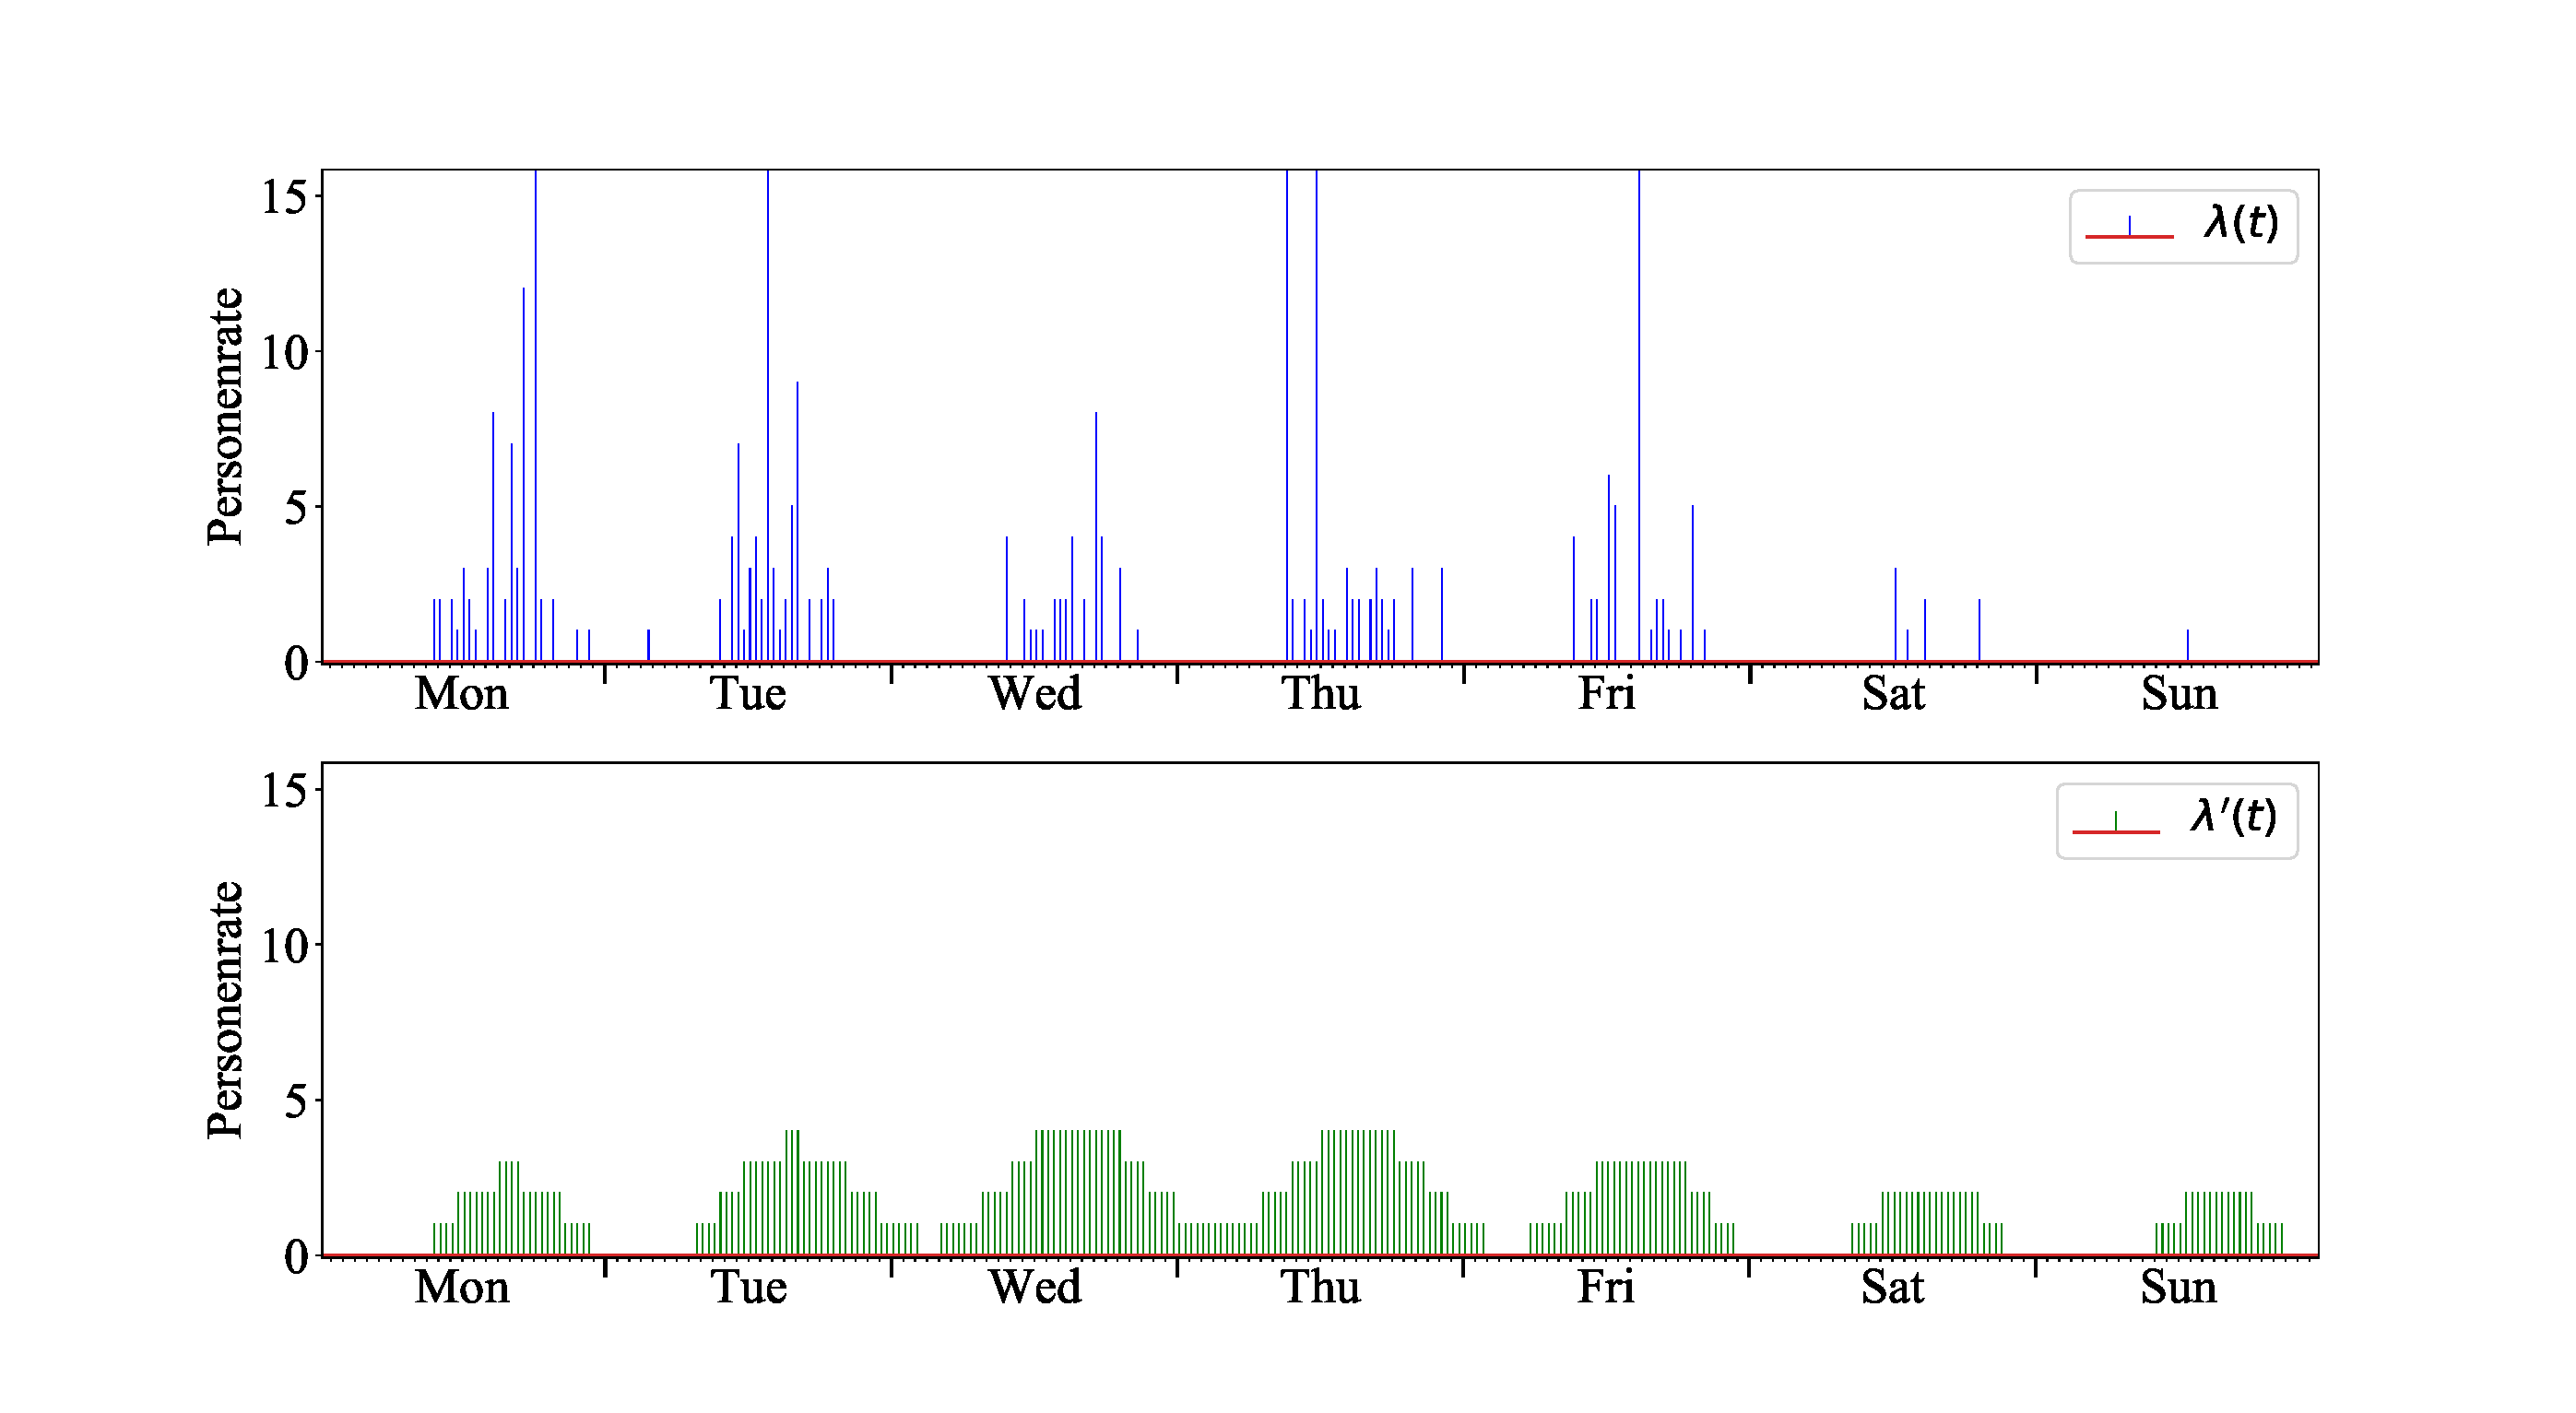
\includegraphics[width=1.0\linewidth]{Abbildungen/evaluation/bin_size_influence_cell_row_23_col_25_float_600}
	\caption{Personenraten einer Beispielzelle des UOL Datensatzes bei einer Intervalldauer von $\Delta t = \SI{600}{\second}$ mit optimaler Modellordnung}
	\label{fig.bin_size_influence_cell_row_23_col_25_float_600}
\end{figure}

Dieser, im Vergleich zu dem quantitativen Modell des Aruba-Datensatzes, hohe Fehler, lässt sich durch die höhere Varianz der einzelnen Wochen innerhalb des UOL-Datensatzes erklären. Jedoch lassen sich auch hier der Tag-Nacht-Rhythmus sowie ein Abflachen der Personenraten während der beiden Wochenendtage erkennen. Die Annahme einer statischen Personenrate von $\lambda_\ind{stat} ' (t) = \mathrm{const}. = 1 $ resultiert in einem Prädiktionsfehler von $\epsilon_\ind{p,stat} = 11.46$. Im Vergleich zum statischen Modell kann also mit einer Modellordnung von $l_\ind{opt} = 2$ eine Verbesserung um 0.7 \% erreicht werden.

Das Modell bei einer Intervalldauer von $\Delta t = \SI{900}{\second}$ ist in \bild{bin_size_influence_cell_row_23_col_25_float_900} dargestellt. 
% Hier Abbildung bin_size_influence_cell_row_23_col_25_float_900.pdf einfügen
\begin{figure}[!h]
	\centering
	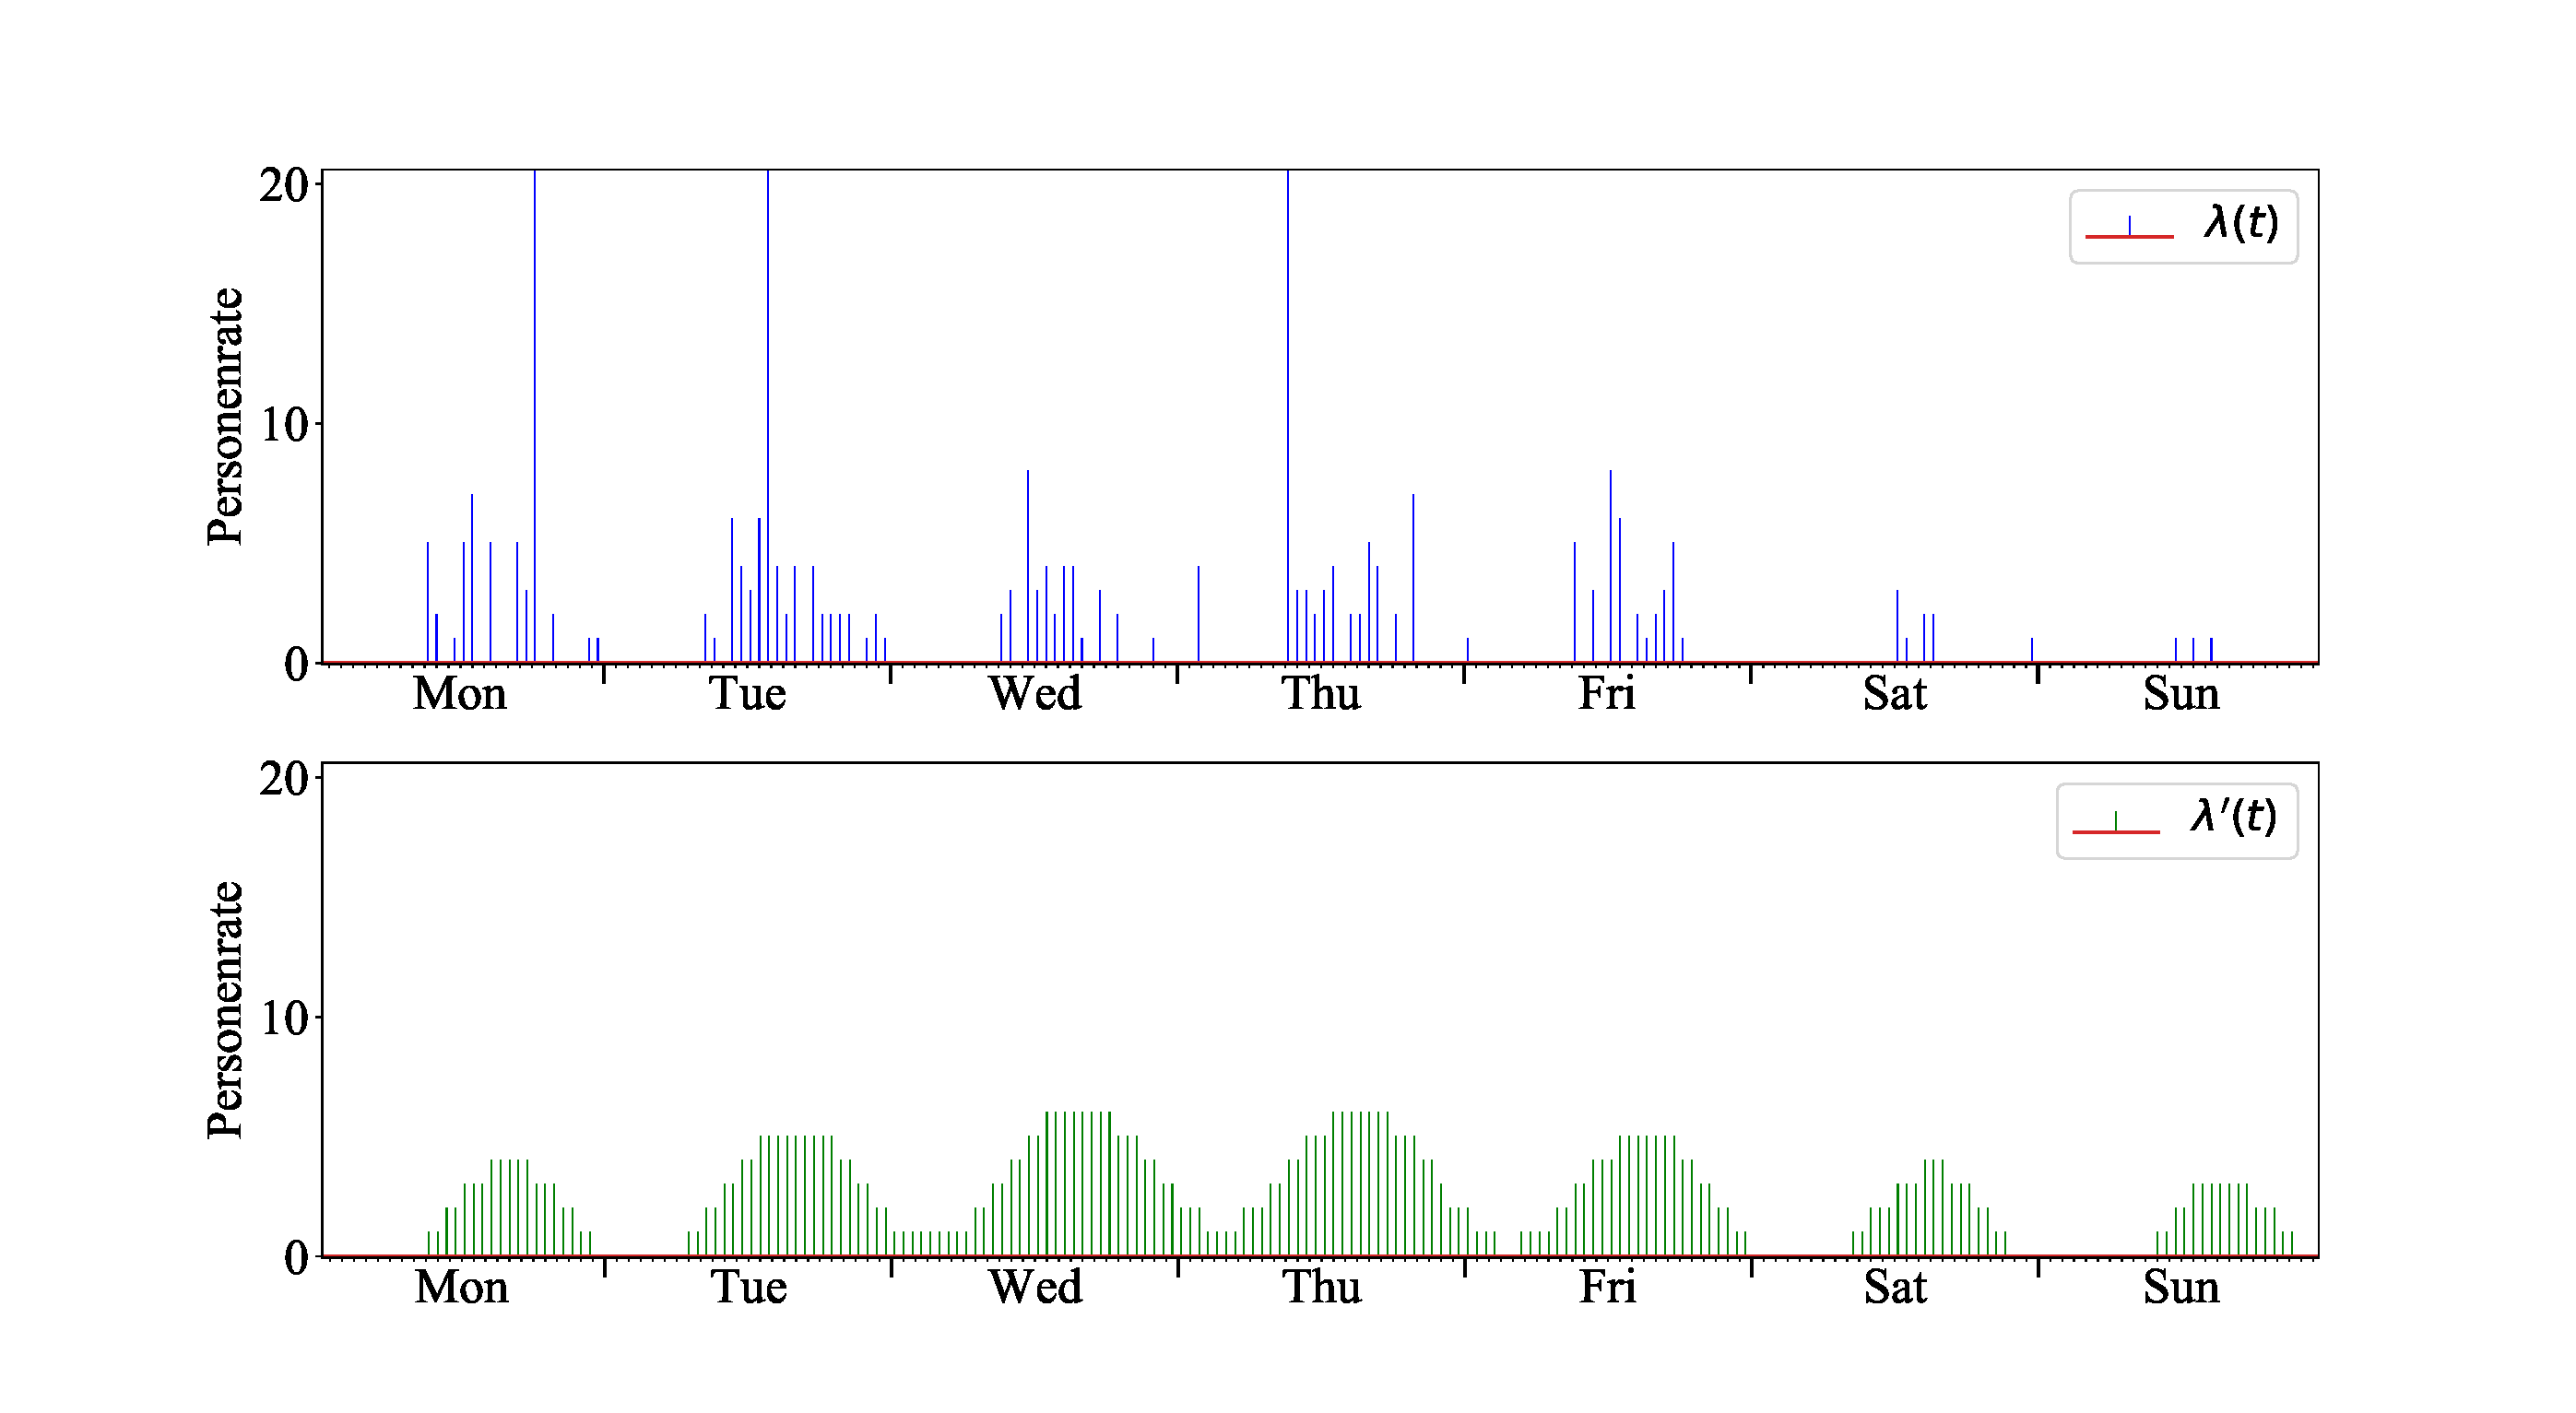
\includegraphics[width=1.0\linewidth]{Abbildungen/evaluation/bin_size_influence_cell_row_23_col_25_float_900}
	\caption{Personenraten einer Beispielzelle des UOL Datensatzes bei einer Intervalldauer von $\Delta t = \SI{900}{\second}$ mit optimaler Modellordnung}
	\label{fig.bin_size_influence_cell_row_23_col_25_float_900}
\end{figure}

Zu erkennen ist, dass die Personenraten $\lambda (t)$ im Vergleich zu \bild{bin_size_influence_cell_row_23_col_25_float_600} höher liegen. Dies ist erneut durch die längere Intervalldauer $\Delta t$ zu erklären. Für $\Delta t = \SI{900}{\second}$ liegt die optimale Modellordnung ebenfalls bei $l_\ind{opt} = 2$, mit einem Prädiktionsfehler von $\epsilon_\ind{p,opt} = 14.51$. Im Vergleich dazu liegt der Prädiktionsfehler des statischen Modells bei $\epsilon_\ind{p,stat} = 14.65$, es konnte also eine Verbesserung um 0.95 \% erreicht werden. \\
In Tabelle \ref{tab.Prädiktionsfehler uol_float} sind die durchschnittlichen Prädiktionsfehler der Zellen des Datensatzes bei verschiedenen Intervalldauern aufgeführt.

\begin{table}[!h]
	\centering
	\caption{Prädiktionsfehler $\epsilon_\ind{p}$ bei unterschiedlichen Intervalldauern  $\Delta t$ (UOL)}\label{tab.Prädiktionsfehler uol_float}
	\vspace*{-3mm}
	\begin{tabular}{lccr}
		\toprule
		Intervalldauer $\Delta t$		& $\epsilon_\ind{p,opt}$	&  $\epsilon_\ind{p,stat}$  & Vergleich $\epsilon_\ind{p,opt}$ zu $\epsilon_\ind{p,stat}$              \\
		\midrule
		\SI{300}{\second}	& 4.80           & 4.83 & -0.63 \% \\
		\rowcolor{Snow2}
		\SI{600}{\second} 	& 6.38           & 6.44 & -0.93 \% \\
		\SI{900}{\second}			& 6.91           & 6.99 & -1.15 \% \\
		\bottomrule
	\end{tabular} 
\end{table}
Verglichen werden erneut die Fehler $\epsilon_\ind{p,opt}$ der Modelle mit einer optimalen Modellordung, demgegenüber gestellt sind die Prädiktionsfehler $\epsilon_\ind{p,stat}$ der statischen Modelle. In die Fehlerermittlung flossen nur Zellen ein, bei welchen in mindestens 5 \% der Intervalle Personendetektionen vorliegen. Unter Berücksichtigung dieser Voraussetzung wurden 205 der insgesamt 3060 Zellen des UOL-Datensatzes zur Fehlermittlung in Tabelle \ref{tab.Prädiktionsfehler uol_float} genutzt. \\
\newpage
Eine Darstellung des über die Umgebung $\mathcal{U}$ gelegten Gitters mit seinen einzelnen Zellen bietet \bild{original_float_data}. Für ein beispielhaftes Zeitintervall $\Delta t_i$ mit einer Dauer von $\Delta t = \SI{600}{\second}$ ist hier für jede Zelle die zugehörige Personenrate $\lambda (t)$ farblich dargestellt. Die entsprechenden Werte der Personenraten $\lambda (t)$ sind farblich kodiert und können der eingezeichneten Farbskala entnommen werden. Zu erkennen ist, dass im vorliegenden Zeitintervall die höchsten Personenraten $\lambda (t)$ innerhalb des linken, oberen Bereiches des Bürogebäudes vorzufinden sind. Außerhalb des Gebäudes finden sich vereinzelt Bereiche mit niedrigen Personenraten (vgl. \bild{original_float_data}).
% caption ändern !
\begin{figure}[!h]
	\centering
	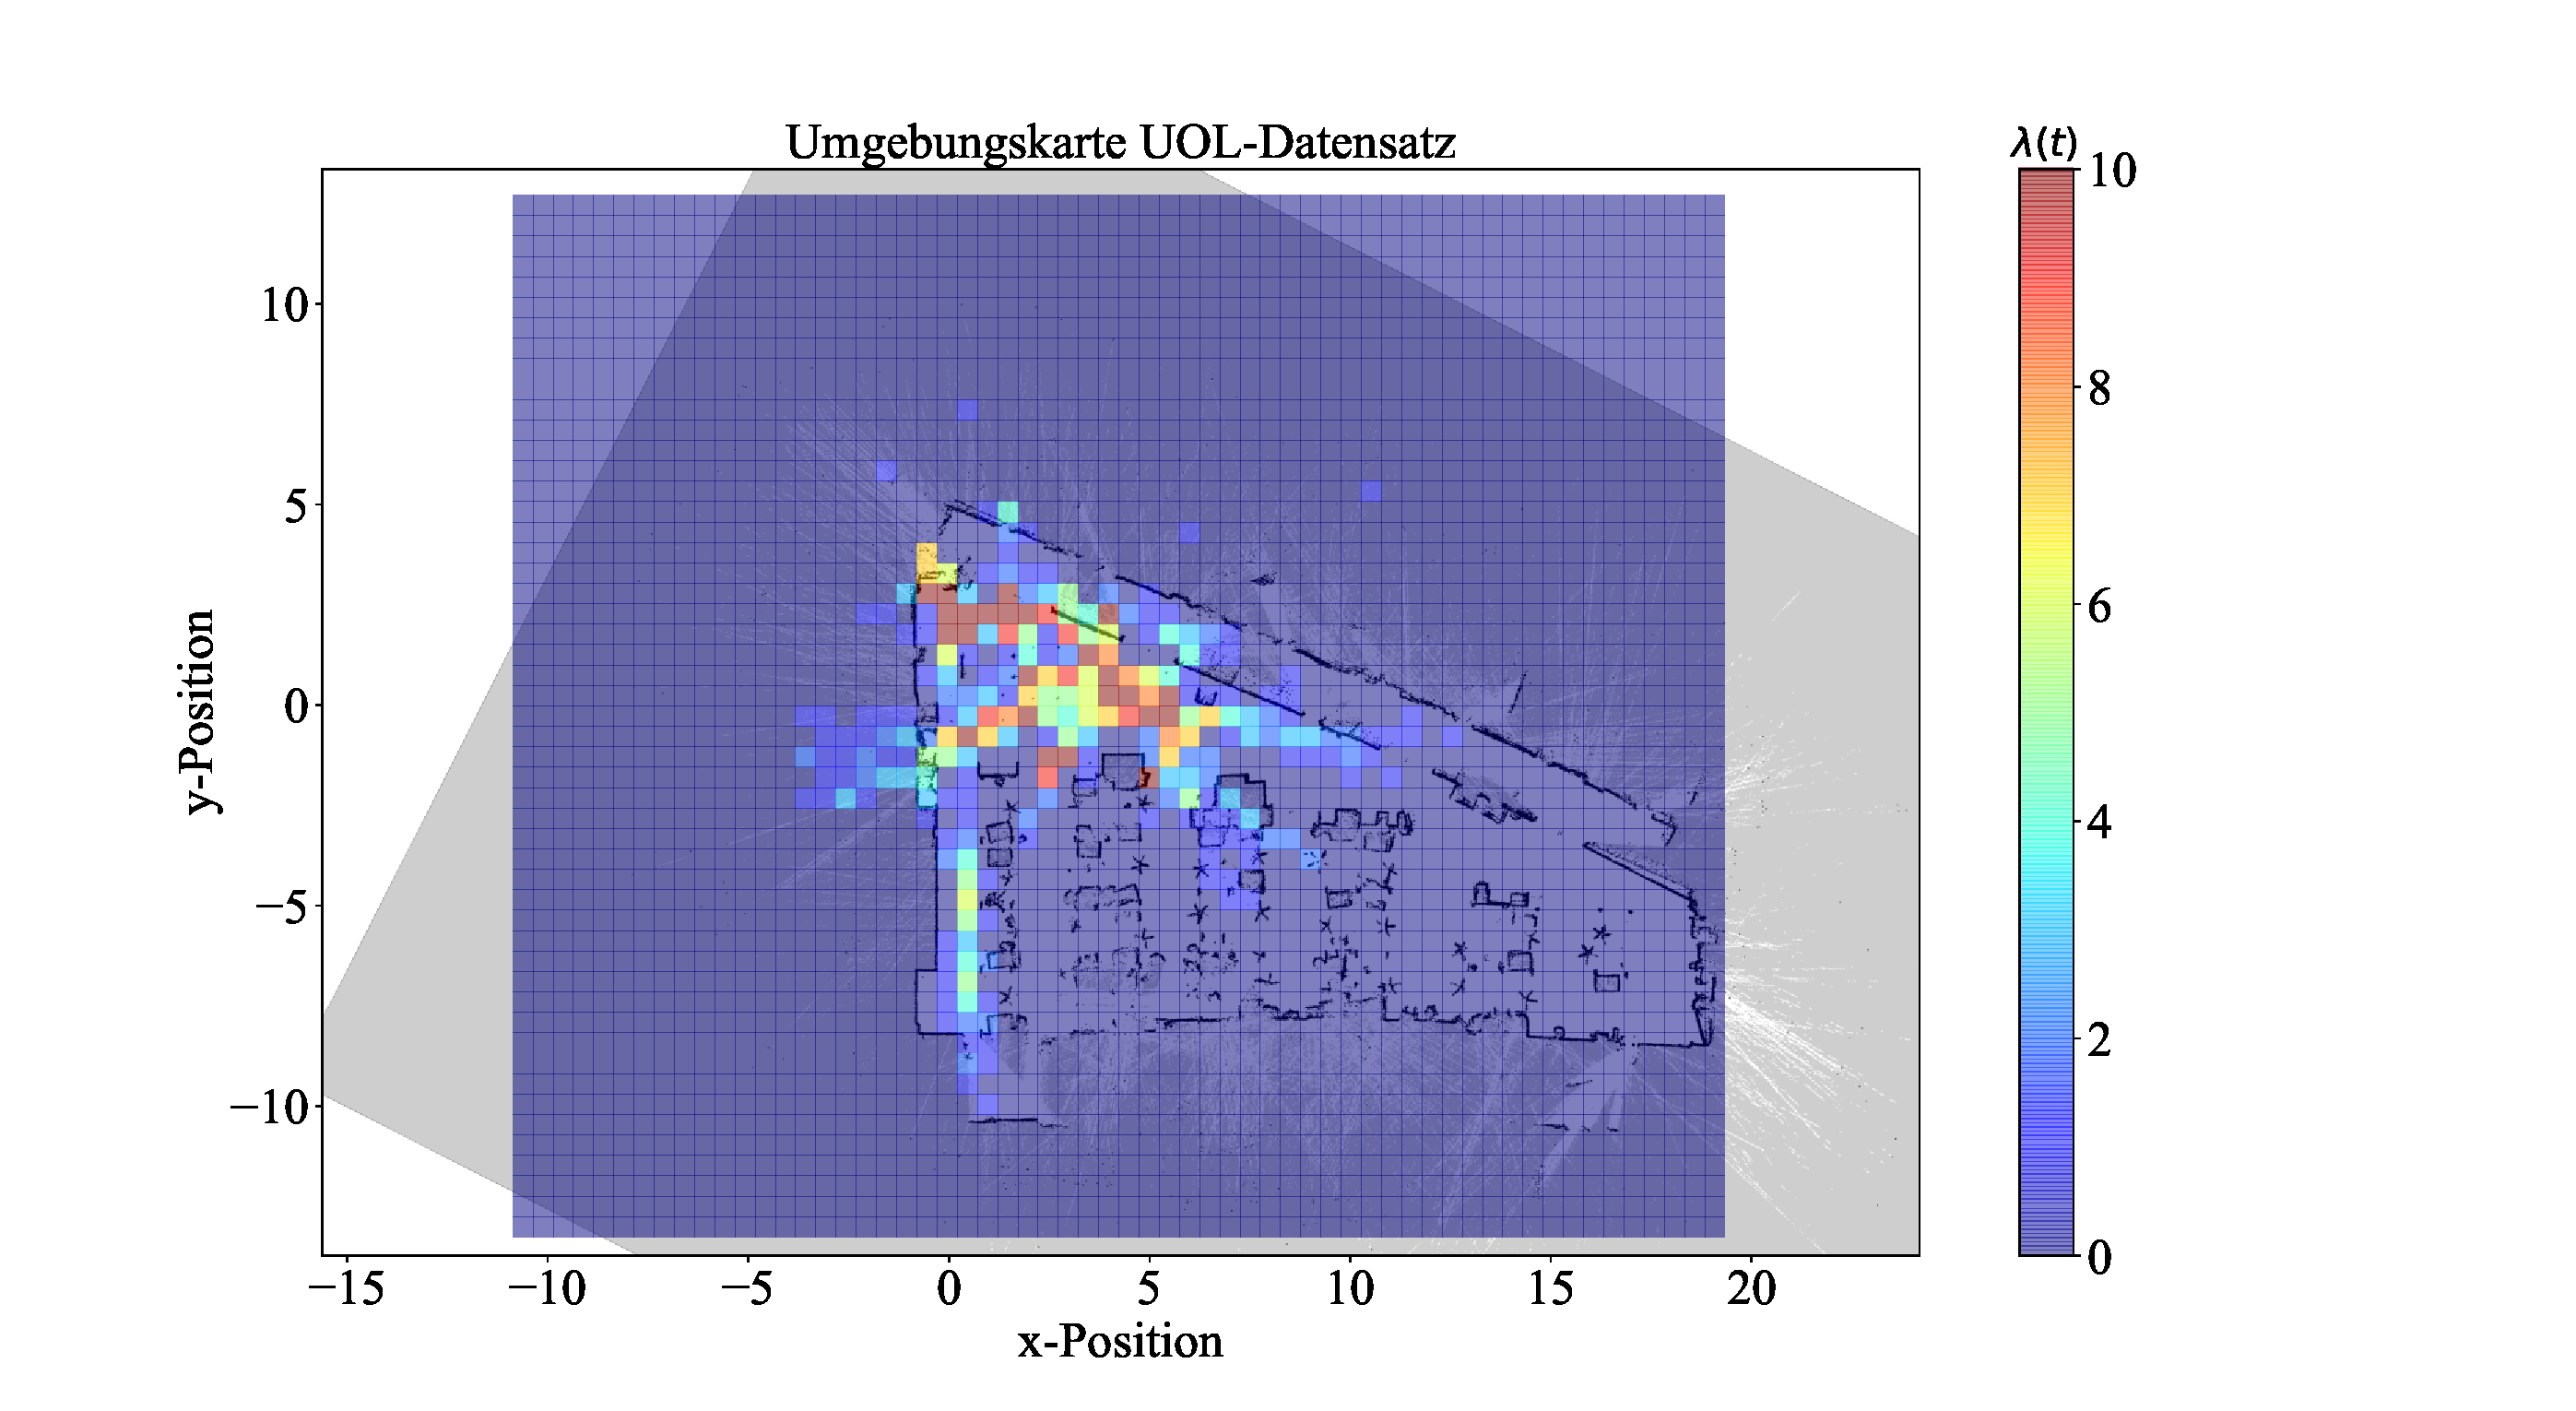
\includegraphics[width=1.0\linewidth]{Abbildungen/evaluation/original_float_data}
	\caption{Tatsächliche Personenraten $\lambda(t)$ innerhalb eines Beispielintervalls $\Delta t_i$}
	\label{fig.original_float_data}
\end{figure}

Ein grafischer Vergleich zwischen den mittels der optimalen Modellordnungen $l_\ind{opt}$ berechneten FreMEn-Modellen und den statischen Modellen der Personenraten $\lambda (t)$ kann mit Hilfe von \bild{float_fremen_vs_static} gezogen werden. \\

\begin{figure}[!h]
	\centering
	\subfigure[Prognostizierte Personenraten $\lambda'(t)$ mit FreMEn-Modellen der Ordnungen $l_\ind{opt}$\label{fig.float_best_prediction}]{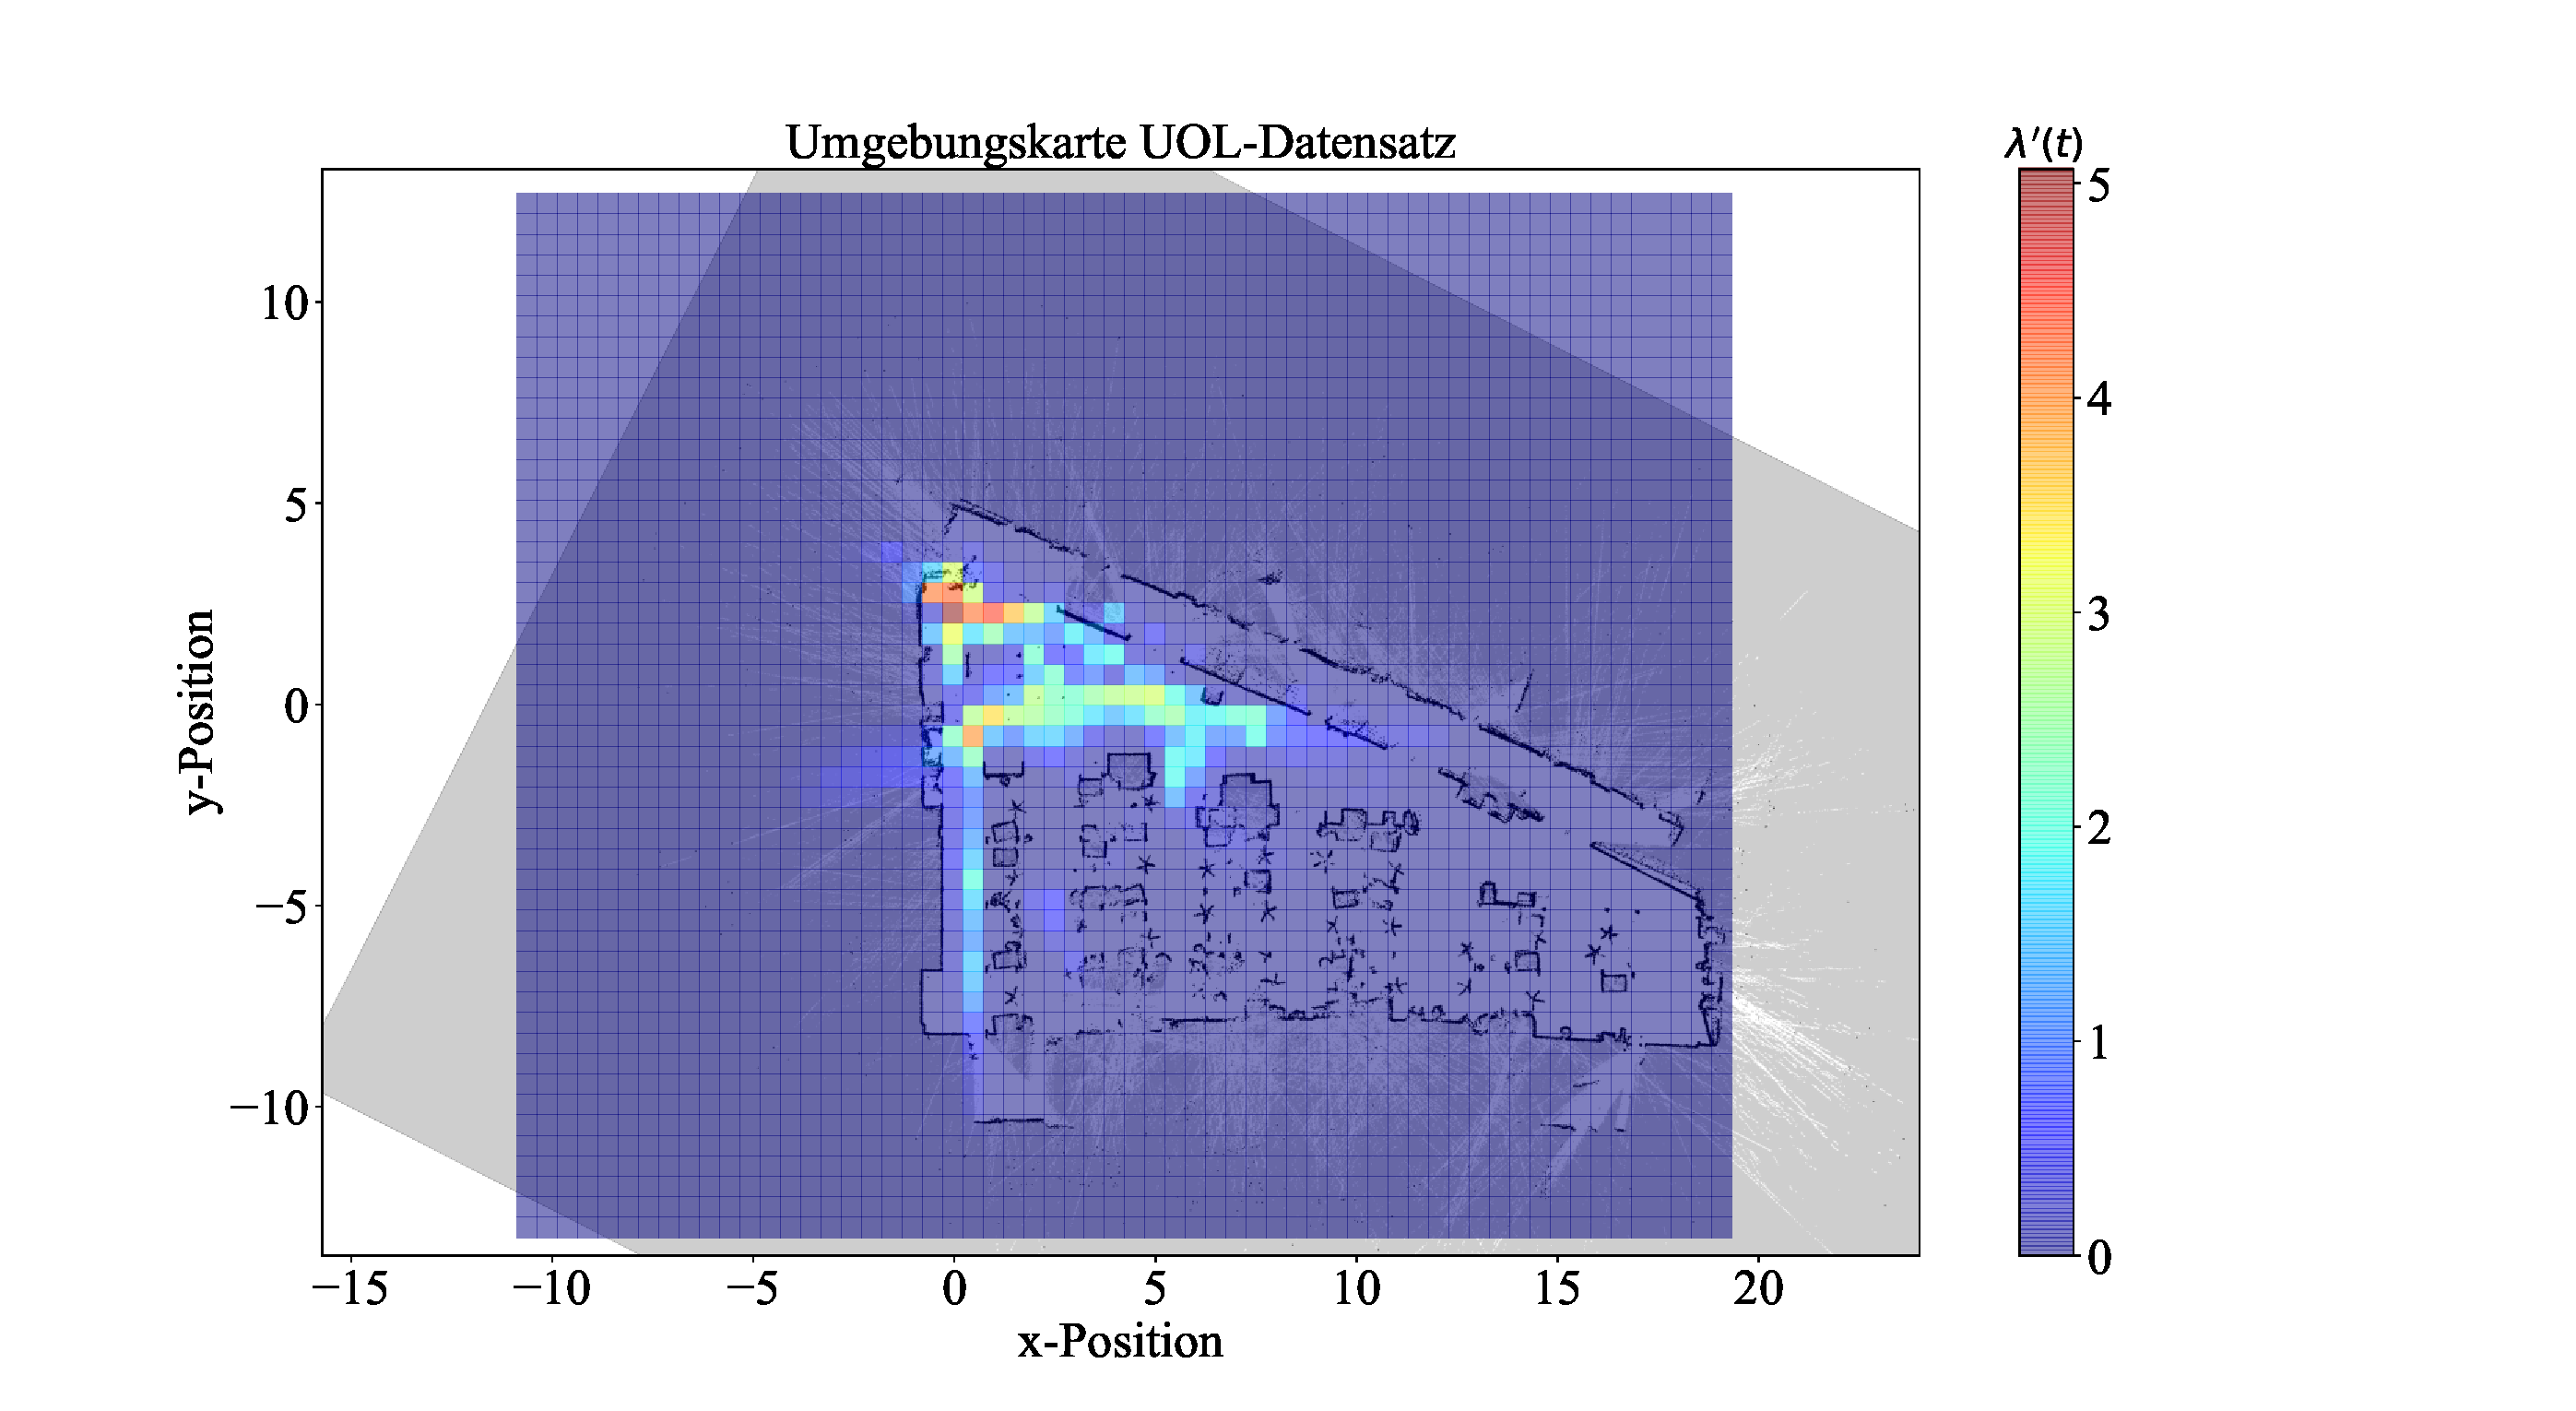
\includegraphics[width=1.0\linewidth]{Abbildungen/evaluation/float_data_best_prediction}}
	
	\subfigure[Prognostizierte Personenraten $\lambda'(t)$ mit statischen Modellen\label{fig.float_static}]{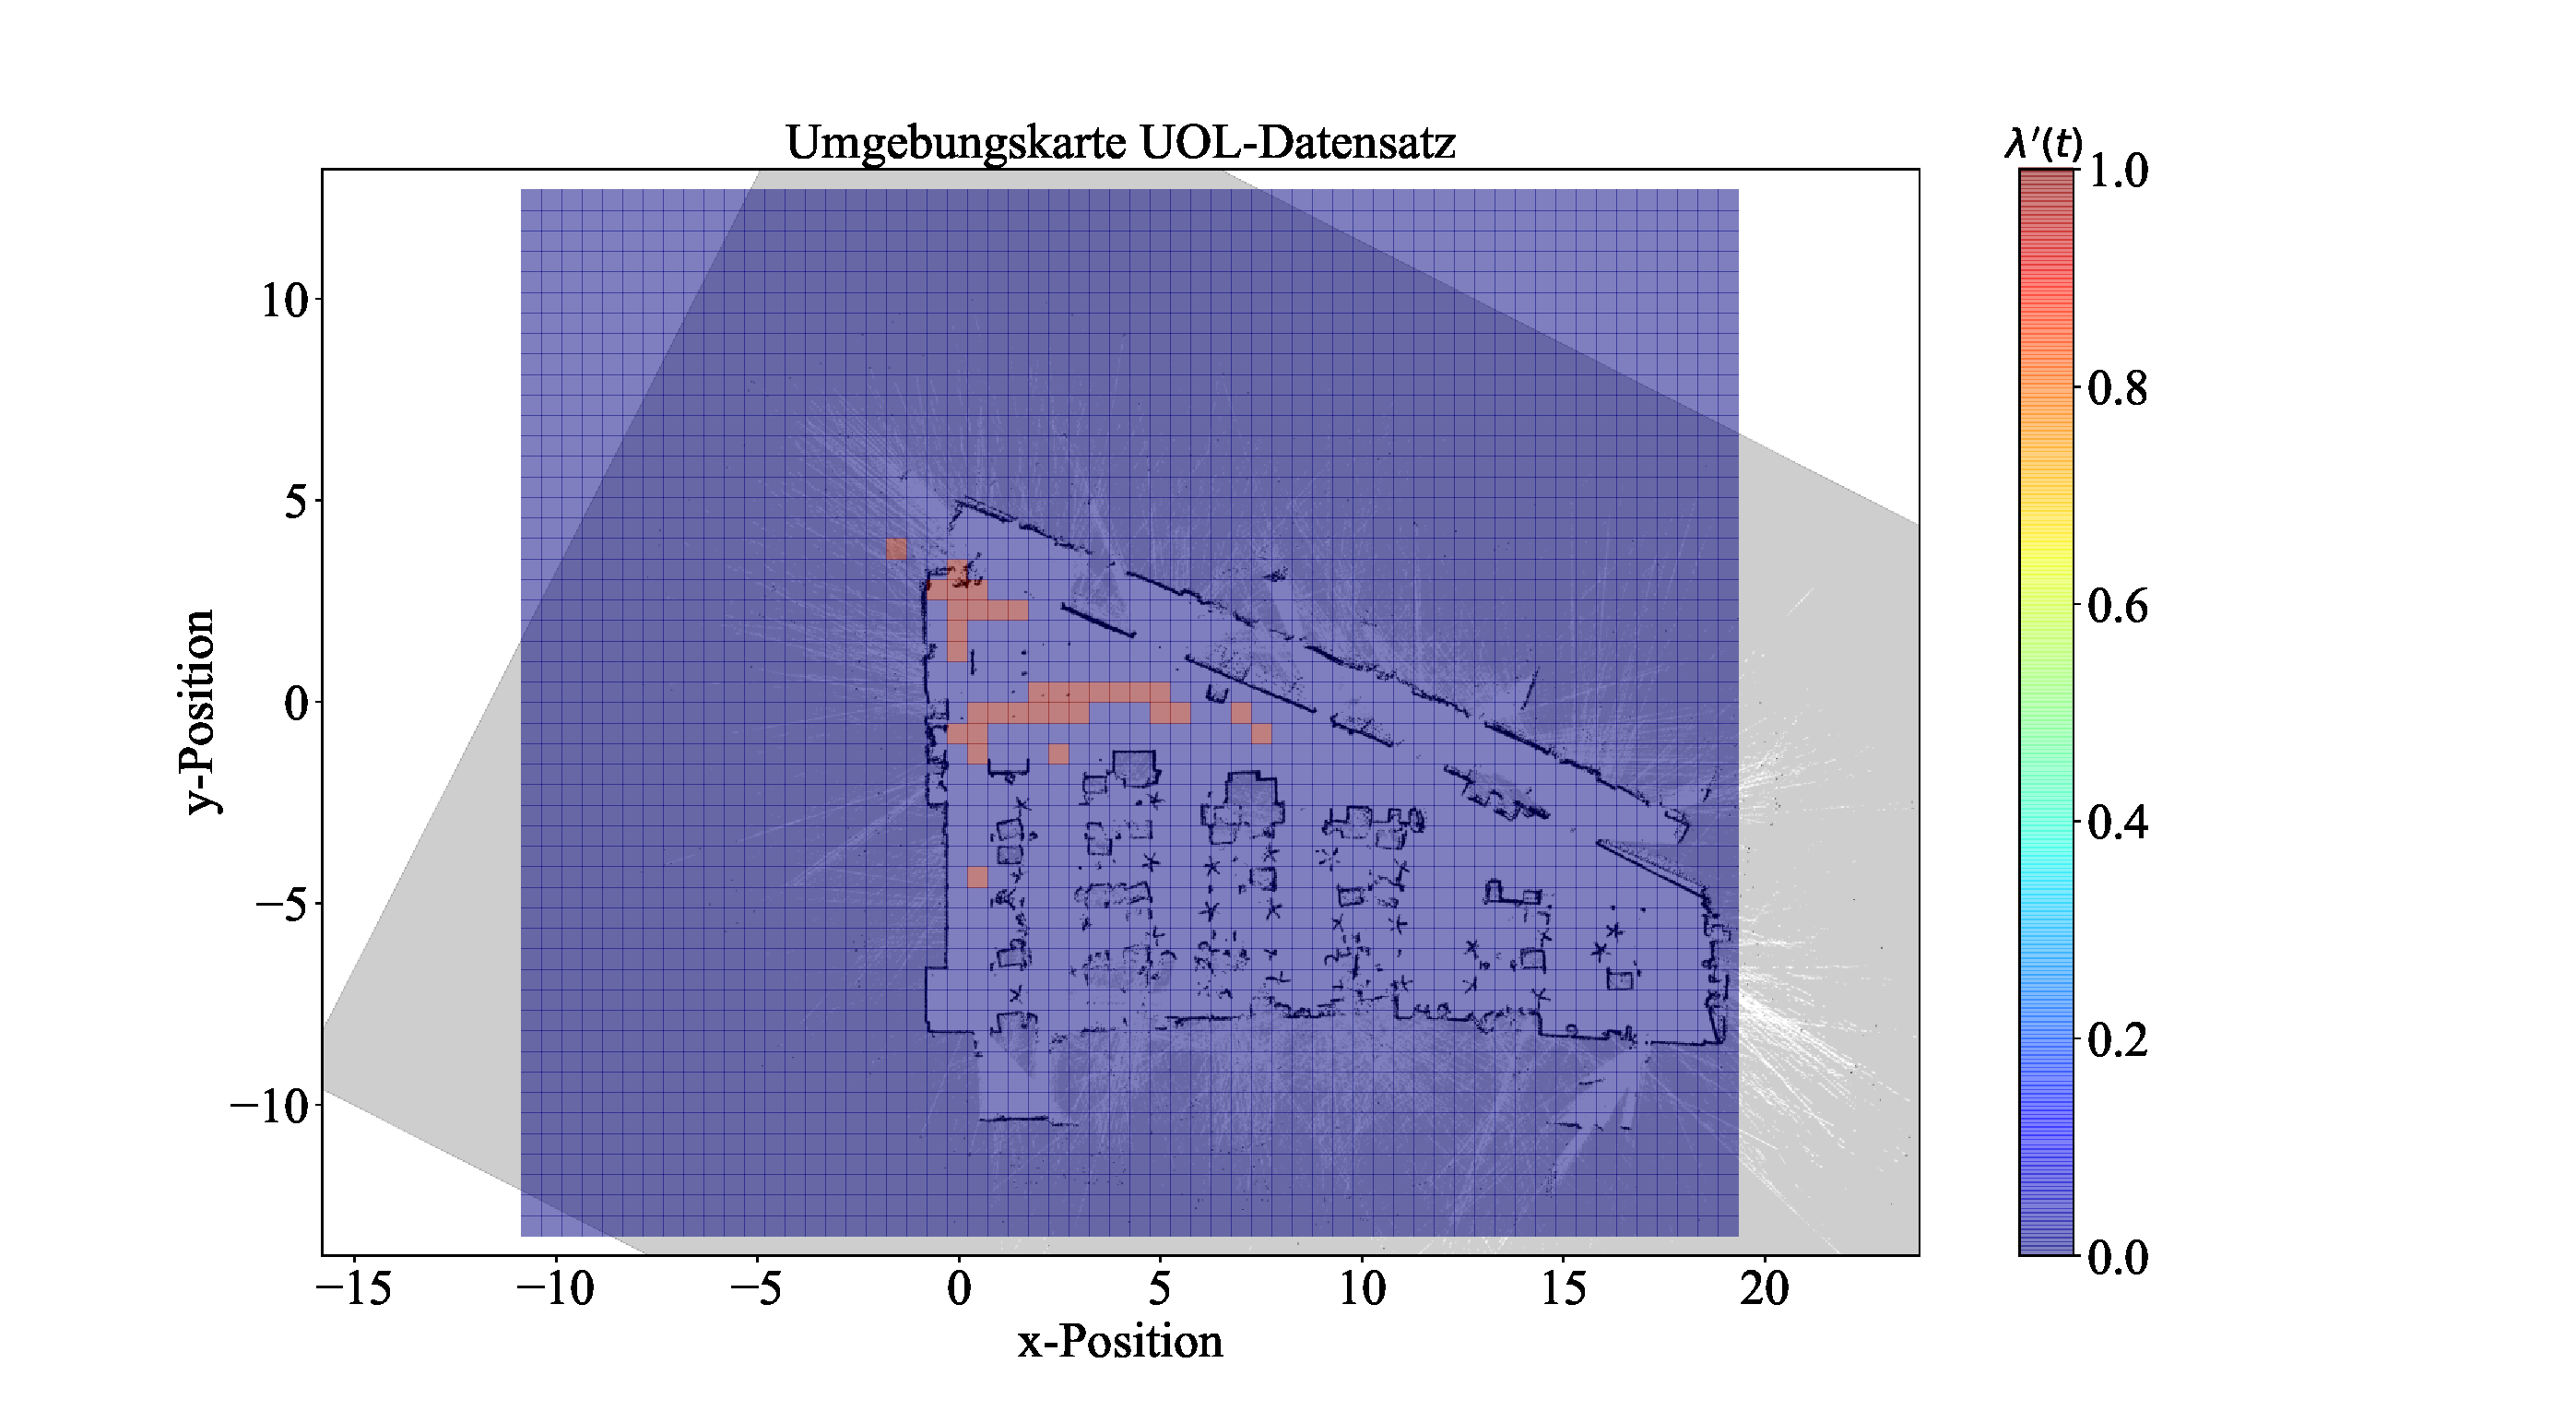
\includegraphics[width=1.0\linewidth]{Abbildungen/evaluation/float_data_static}}
	\caption{Vergleich von FreMEn-Modellen mit statischen Modellen für den quantitativen Fall}
	\label{fig.float_fremen_vs_static}
\end{figure}

Zu erkennen ist, wie schon im Fall binärer Modelle (Abschnitt \ref{sec.Binäres Modell}), dass die FreMEn-Modelle erneut nur in einem Teil der Zellen, in welchen innerhalb des Zeitintervall $\Delta t_i$ Personenraten vorlagen, diese auch prognostizieren. Der Trend der Konzentration hoher Personenraten $\lambda (t)$ innerhalb der Zellen der oberen linken Ecke des Bürogebäudes wird jedoch abgebildet. Vereinzelt werden auch außerhalb des Bürogebäudes Zellen mit Personenraten größer als null prognostiziert. Im Vergleich zu \bild{original_float_data} mit einer maximalen Personenrate von $\lambda_\ind{max} (t) = 10$ beträgt die maximale prognostizierte Personenrate mittels der FreMEn-Modelle $\lambda'_\ind{max} (t) = 5$ (vgl. Bild \ref{fig.float_best_prediction}). Betrachtet man die prognostizierten Personenrate der statischen Modelle (Bild \ref{fig.float_static}), so ergeben sich dort die maximalen prognostizierten Personenraten zu $\lambda'_\ind{max} (t) = 1$. Die Zellen, für welche Personenraten größer als null prognostiziert werden, befinden sich in der linken, oberen Ecke des Bürogebäudes. Verglichen mit den tatsächlichen Personenraten $\lambda (t)$ aus \bild{original_float_data} bilden die FreMEn-Modelle diese deutlich genauer ab als die statischen Modelle.

